\chapter{排序}\label{Sec:Chapter:Sort}

\section{概述}
在本章中我们将学习几个排序的算法,所谓排序算法就是将集合中的元素按顺序排列。
将一组元素排序的问题是第一个广泛研究的计算机科学问题。已知最好的
\emph{分而治之}的许多算法设计范例都是排序算法。在20世纪60年代,当商业
数据处理大规模使用自动化时,在安装计算机的地方排序程序是运行最多的程序。
一个软件公司靠着更好的排序程序在行业内能领先好几年。以今天的硬件水品,
排序性能的关键有所改变。在20世界60年代,低速存储器(磁带或磁盘)和
主存之间的传输速度是主要的性能瓶颈。主存一般只有100,000字节,而要排序
的文件大多比这要大一个数量级以上。主要的研究都是适合这种类型的排序算法。
现在,主存容量增长了1,000倍(也就是约100MB),或者高达GB
\footnote{译注:今天GB已经是标准配置了}。所以大多数文件都能装入主存了。

有好几个原因要学习排序算法。首先,经常需要排序。以字母顺序排序电话簿或
字典以使他们更容易使用,在计算机中操作大容量有序的集合比不无序的要容易。
其次,人们开发了如此多的排序算法(本章将讲解很多种),而且学习很多排序
算法会给你深刻的影响,即你可以从很多方面来考虑同样的一个问题。如何改进
一个给出的算法,如何在多个算法之间取舍,本章对算法的讨论一定会让你更清楚
的理解这两个问题。最后,排序是少数几个我们能简单的推导出最坏情况和平均
行为的强低限的问题。说底限是强的是指已经有算法近似的达到了最小的工作量。
因而我们已经根本上最优化了排序算法。

在大多数算法的描述中,我们假定要排序的集合存储在数组中,所以访问任意位置
元素的时间都是常数;称为\emph{随机访问random access}。但是,有些算法对于
排序文件和链表也是很有用的。当集合仅以顺序方式访问时,我们使用术语序列sequence,
来强调集合的结构可能是顺序文件或是链表,也可以是数组。如果数组的索引定义
为$0,\cdots, n-1$,则数组的\emph{范围range}或\emph{子范围subrange}是指两个
给定索引之间连续的数组项,一般写做first和last,$0\leq first$,$last\leq n-1$。如果
$last<first$,称范围是\emph{空}。

我们假设集合中每一个要排序的元素都包含一个标识,叫做\emph{关键字key},这是一个
线性集合的元素,两个关键字可以比较以决定他们哪一个大或是两者相等。我们
总是以非递减顺序排序关键字。集合中的每一个元素都可以包含除key之外的信息。
当在排序过程中,key重排列之后,相应的信息也会跟着重排列,但是有时我们仅
关心key,而不显示的给出数组项剩下的信息。

\ref{Sec:InsertSort}小节到\ref{Sec:ShellSort}小节考虑的算法都是只通过比较
关键字(和复制他们)进行排序的一类算法,这类算法必须不对关键字做其他操作。
我们称这些是“通过比较关键字排序的算法”,或简称“基于比较的算法”。分析这类
算法主要的工作是计算比较关键字的次数。在\ref{Sec:LowerBoundsForSortingByComparisonOfKeys}
小节建立了这类算法需要的比较次数的低限。\ref{Sec:RadixSorting}小节讨论可以
对关键字使用其他的排序算法,以及不同的度量工作量的方法。

本章的算法叫做\emph{内部排序internal sorts}因为假设数据都在计算机高速随机访问
的主存中。当集合数据量过大而不能放在主存中时性能问题的焦点就有所不同。对
存储在外部、低速存储设备中且对数据的访问有约束的数据集合排序算法称为
\emph{外部排序external sorts}。参看本章后面的Notes和References找到这类算法更多的信息。

当分析排序算法时,我们将考虑他们将使用多少额外空间(超过输入数据的那一部分)。
如果额外空间的大小相对与输入是一个常数,算法称为\emph{in place}。

为了帮助算法更清楚,我们使用Element和Key作为类型标识符,但是认为Key是一个
数值类型,我们对Key使用“$=$,$\neq$,$<$”等关系运算符。当书中使用类似
“E[i].key<x”关键字比较表达式时,如果实际的类型是非数值的(例如\textbf{String}),
Java程序提供了语法来调用方法,比如“less(E[i].key, x)”。许多语言都是这样。

\emph{Java语言提示:}通过Java中的Comparable接口,可以写一个能比较各种关键字
类型的过程,类型Key必须体换成关键字Comparable。细节在附录A给出。复习一下
Java中的数组申明为Element[] arrayName。

\section{插入排序}\label{Sec:InsertSort}
从插入排序开始是一个很好的选择,因为它的思想是很自然和很一般的,而且计算
它的最坏时间和平均行为时间也很简单。它也是我们在\ref{Sec:ShellSort}小节
讨论的更快的算法要用到的部分。

\subsection{策略}
\begin{figure*}[!t]
    \centering
    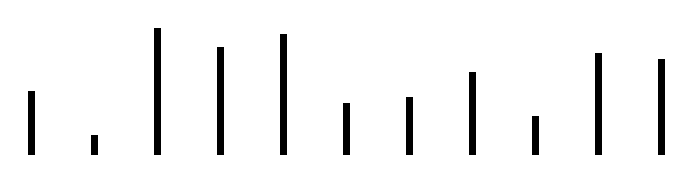
\begin{tikzpicture}[scale=0.8, place/.style={circle,draw, minimum size=5mm}]
        \filldraw[fill=black] (0,0) rectangle (0.1,1);
        \filldraw[fill=black] (1,0) rectangle (1.1,0.3);
        \filldraw[fill=black] (2,0) rectangle (2.1,2);
        \filldraw[fill=black] (3,0) rectangle (3.1,1.7);
        \filldraw[fill=black] (4,0) rectangle (4.1,1.9);
        \filldraw[fill=black] (5,0) rectangle (5.1,0.8);
        \filldraw[fill=black] (6,0) rectangle (6.1,0.9);
        \filldraw[fill=black] (7,0) rectangle (7.1,1.3);
        \filldraw[fill=black] (8,0) rectangle (8.1,0.6);
        \filldraw[fill=black] (9,0) rectangle (9.1,1.6);
        \filldraw[fill=black] (10,0) rectangle (10.1,1.5);
    \end{tikzpicture}
    \caption{未排序元素}
    \label{Fig:UnsortedElements}
\end{figure*}

\begin{figure*}[!t]
    \centering
    \begin{tikzpicture}[scale=0.8, place/.style={circle,draw, minimum size=5mm}]
        \filldraw[fill=black] (0,0) rectangle (0.1,0.3);
        \filldraw[fill=black] (1,0) rectangle (1.1,1);
        \filldraw[fill=black] (2,0) rectangle (2.1,1.7);
        \filldraw[fill=black] (3,0) rectangle (3.1,1.9);
        \filldraw[fill=black] (4,0) rectangle (4.1,2);

       \draw[->] (5, 2.5)node[right]{x}-- (5, 0.9);

        \filldraw[fill=black] (5,0) rectangle (5.1,0.8);
        \filldraw[fill=black] (6,0) rectangle (6.1,0.9);
        \filldraw[fill=black] (7,0) rectangle (7.1,1.3);
        \filldraw[fill=black] (8,0) rectangle (8.1,0.6);
        \filldraw[fill=black] (9,0) rectangle (9.1,1.6);
        \filldraw[fill=black] (10,0) rectangle (10.1,1.5);
        \draw (0, -0.5cm+4pt) -- (0cm,-0.5cm-4pt) node{};
        \draw (4, -0.5cm+4pt) -- (4cm,-0.5cm-4pt) node{};
        \draw (6, -0.5cm+4pt) -- (6cm,-0.5cm-4pt) node{};
        \draw (10, -0.5cm+4pt) -- (10cm,-0.5cm-4pt) node{};
        \node at(2,-0.5) {-已经排序的-};
        \node at(8,-0.5) {-还没有检查的-};
    \end{tikzpicture}
    \caption{部分排序元素}
    \label{Fig:PartiallySortedElements}
\end{figure*}

\begin{figure*}[!t]
    \centering
    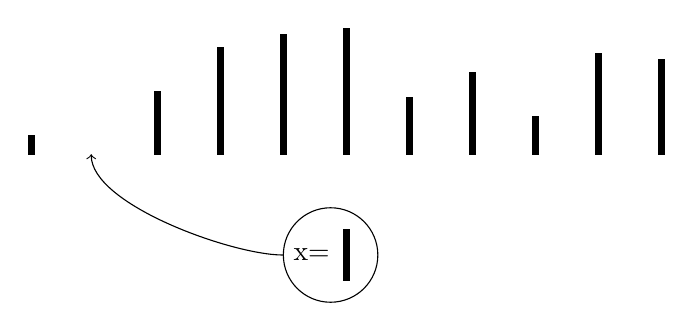
\begin{tikzpicture}[scale=0.8, place/.style={circle,draw, minimum size=5mm}]
        \filldraw[fill=black] (0,0) rectangle (0.1,0.3);

        \filldraw[fill=black] (2,0) rectangle (2.1,1);
        \filldraw[fill=black] (3,0) rectangle (3.1,1.7);
        \filldraw[fill=black] (4,0) rectangle (4.1,1.9);
        \filldraw[fill=black] (5,0) rectangle (5.1,2);

        \filldraw[fill=black] (6,0) rectangle (6.1,0.9);
        \filldraw[fill=black] (7,0) rectangle (7.1,1.3);
        \filldraw[fill=black] (8,0) rectangle (8.1,0.6);
        \filldraw[fill=black] (9,0) rectangle (9.1,1.6);
        \filldraw[fill=black] (10,0) rectangle (10.1,1.5);

        \draw (4.5, -1.6) node{x=};
        \filldraw[fill=black] (5,-2) rectangle (5.1,-2+0.8);
        \node  (x) at (4.8,-1.6) [circle,draw,minimum size=12mm] {};
        \draw [->] (x.west) .. controls +(left:8mm) and +(down:8mm) .. (1,0);
    \end{tikzpicture}
    \caption{将x插入道正确的位置}
    \label{Fig:InsertionOfXInProperOrder}
\end{figure*}

我们从有n个元素以任意序列的E开始,如图\ref{Fig:UnsortedElements}。(插入
排序可以用于关键字是任意线型顺序集合的情况,但是对于小棍的插图,将棍的高
想象成关键字。)

假设我们已经将序列的一些小段排序了。图\ref{Fig:PartiallySortedElements}显示
了一个左边的5个已经排完序的快照。下一步就是通过把剩下的元素插入到它正确的
位置来增加已排序列的长度。

令x是要插入已排序列的下一个元素,就是说,x是未检查段的最左边元素。第一步我
们把x“搬走”(就是将它拷贝到局部变量),在x的位置留一个空位。然后我们依次
将x与空位左边的元素比较,只要x比左边的元素大,我们就这个元素搬到空位,留下
一个新的空位。就是说,空位向左移动了一步。重复这个过程直到,我们没有元素移
到空位中,或是当前空位左边的元素小于或等于x。将x插入空位,如图
\ref{Fig:InsertionOfXInProperOrder}。为了让算法开始,我们只需要将第一个元素
看作是一个有序段就可以了。现在我们将这些步骤规范化成移个过程,我们假定序列
是一个数组;当然对于list或其他的线性序列结构也是可以的。

\begin{figure*}[!t]
\colorbox[rgb]{0.9, 0.9, 0.9}{int shiftVac(Element[] E, int vacant, Key x)}

\emph{preconditions:}vacant 是非负的。

\emph{postconditions:}令 xLoc是返回的值。则:
\begin{enumerate}
\item E中的索引小于xLoc的元素在它原来的地方,且key都小于或等于x。
\item E中的元素位置在xLoc+1直到vacant的,大于x的元素都将在shiftVac调用之后把位置移动一格。
\end{enumerate}
\caption{shiftVac的规范}
\label{Fig:SpecificationsForShiftVac}
\end{figure*}

\subsection{算法和分析}
现在我们仔细的实现排序过程。让子例程shiftVac(E, vacant, x)做搬运的工作,直
到把空位移动到按顺序x应该在的地方。过程返回空位的索引,叫做xLoc。Precondition
和postcondition都在图\ref{Fig:SpecificationsForShiftVac}中。换句话说,
shiftVac完成图\ref{Fig:PartiallySortedElements}到图\ref{Fig:InsertionOfXInProperOrder}
的转换。现在insertionSort可以一直调用shiftVac,使得左边的段越来越长,直到
所有的元素都在有序段中。

shiftVac过程是一个典型的\emph{普通搜索例程}(定义\ref{Def:GeneralSearch})。
如果没有数据了,fail;否则查找一个元素,如果它是我们要找的元素,成功;否则
继续没有检查过的元素。因为有两种结束情况,可以用一个\textbf{while}循环来表示,
再使用\textbf{break}对于一种或多种结束情况。递归形式是直接的。

\begin{lstlisting}[language={Java},keywordstyle=\color{blue!70}, commentstyle=\color{red!50!green!50!blue!50}]
    int shiftVacRec(Element[] E, int vacant, Key x)
    {
        int xLoc;
    1:  if(vacant==0)
    2:      xLoc= vacant;
        else
    3:      if(E[vacant-1].key<=x)
    4:          xLoc=vacant;
    5:      else
            {
    6:          E[vacant]= E[vacant-1];
    7:          xLoc=shiftVacRec(E, vacant-1,x);
            }
    8:  return xLoc;
    }
\end{lstlisting}


为了验证第7行的递归的正确性,我们注意到递归过程在一个更小的范围内工作,
而且它的第2个元素是非负的,所以是满足precondition(图\ref{Fig:SpecificationsForShiftVac}
中的)的。(你可以检查调用链来论证vacant-1为什么是非负的--它为什么不是负的呢?)
正确性是显然的,如果我们可以假定第7行的递归完成了它的目标的话。

尽管shiftVacRec过程非常简单,如果我们想象一下$E$的第n个元素插入时候的活动跟踪情况,
算一下递归的深度或是堆栈的深度可能增长到规模n。这对于很大的n是不可接受的。因此
这种情况下,当让所有的事情都工作正常之后,递归必须改成迭代。(试图优化不能工作的
程序是徒劳。)目的与其说是为了节约时间不如说是为了节约空间。实际上如果打开优化,
许多编译器将自动执行这个转换过程。下面的完整算法把包含了shiftVac的迭代版本。

\begin{algorithm}
插入排序

{\textbf{\emph{Input:}}}数组E,数组的大小。索引从0到n-1。

{\textbf{\emph{Output:}}}E,其元素是升序。

{\textbf{\emph{Remark:}}}shiftVac子例程的规范在图\ref{Fig:SpecificationsForShiftVac}中给出。

\end{algorithm}
\begin{lstlisting}[language={Java},keywordstyle=\color{blue!70}, commentstyle=\color{red!50!green!50!blue!50}]
    void insertionSort(Element[]E, int n){
        int xindex;
        for(xindex=l; xindex<n; xindex++){
            Element current= E[xindex];
            Key x=current.key;
            int xLoc= shiftVac(E, xindex, x);
            E[xLoc]=current;
        }
        return;
    }
    int shiftVac(Element[]E, int xindex, Key x){
        int vacant, xLoc;
        vacant= xindex;
        xLoc=0; // `假定失败`
        while(vacant>0){
            if(E[vacant-1].key<=x){
                xLoc=vacant; // `成功`
                break;
            }
            E[vacant]=E[vacant-1];
            vacant--;
        }
        return xLoc;
    }
\end{lstlisting}

\subsubsection{最坏情况复杂度}
为了分析,我们使用i代表xindex。对于每一个i的值,关键字比较的最大次数是i
(在一次shiftVac的迭代调用中,或是shiftVacRec的顶层递归 中)。则总数是
\begin{displaymath}
W(n)\leq \sum_{i=1}^{n-1} i=\frac{n(n-1)}{2}
\end{displaymath}
注意,我们已经建立了最坏情况的上界;花点时间来验证对输入确实有n(n-1)/2次
关键字比较。一种最坏情况是当关键字是颠倒顺序的时候(就是说是递减的时候)。
所以
\begin{displaymath}
W(n)=\frac{n(n+1)}{2}\in \Theta(n^2)
\end{displaymath}

\subsubsection{平均行为}
\begin{figure*}[!t]
    \centering
    \centering
    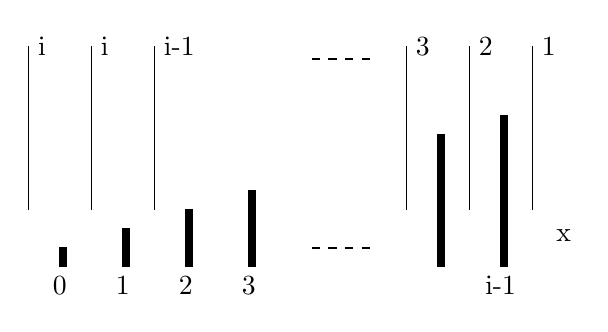
\begin{tikzpicture}[scale=0.8, place/.style={circle,draw, minimum size=5mm}]
        \draw (-0.5, 3.5)node[right]{i}-- (-0.5, 0.9);
        \filldraw[fill=black] (0,0)node[anchor=north]{0} rectangle (0.1,0.3);
        \draw (0.5, 3.5)node[right]{i}-- (0.5, 0.9);
        \filldraw[fill=black] (1,0)node[anchor=north]{1} rectangle (1.1,0.6);
        \draw (1.5, 3.5)node[right]{i-1}-- (1.5, 0.9);
        \filldraw[fill=black] (2,0)node[anchor=north]{2} rectangle (2.1,0.9);
        \filldraw[fill=black] (3,0)node[anchor=north]{3} rectangle (3.1,1.2);

        \draw (5.5, 3.5)node[right]{3}-- (5.5, 0.9);
        \filldraw[fill=black] (6,0) rectangle (6.1,2.1);
        \draw (6.5, 3.5)node[right]{2}-- (6.5, 0.9);
        \filldraw[fill=black] (7,0)node[anchor=north]{i-1} rectangle (7.1,2.4);
        \draw (7.5, 3.5)node[right]{1}-- (7.5, 0.9);
        \draw[thick,dash pattern=on 3pt off 3pt] (4, 0.3) --(5, 0.3);
        \draw[thick,dash pattern=on 3pt off 3pt] (4, 3.3) --(5, 3.3);
        \draw (8, 0.5)node{x};
    \end{tikzpicture}
    \caption{决定x的位置需要的比较次数}
    \label{Fig:CompareCountOfDecidedXPostion}
\end{figure*}
我们假定输入关键字的所有排列都是等概率的。我们首先将决定将一个新关键字插
入到原来已经排序好的片段中需要多少次关键字比较,就是以任意i(用于xindex)
调用一次shiftVac会有多少次比较。为了简化分析,我们假设关键字是不同的。
(分析过程十分类似与第一章做对序列查找做的分析。)

有i+1个位置可能放置x。图\ref{Fig:CompareCountOfDecidedXPostion}展示了插入
的位置决定了要做多少次比较。

x属于任一位置的概率是1/(i+1)。(这依赖于一个事实,即算法之前不知道x的
任何信息。如果算法事先知道关于x的信息,,我们不必假设x对于每一个x的值都
有相等的概率。)因此在shiftVac中找到第i个元素的平均比较次数是
\begin{displaymath}
\frac{1}{i+1}\sum_{j=1}^i+\frac{1}{i+1}i=\frac{i}{2}+\frac{i}{i+1}=\frac{i}{2}+1-\frac{1}{i+1}
\end{displaymath}
现在对于所有的n-1次插入,
\begin{displaymath}
A(n)=\sum_{i=1}^{n-1}=(\frac{i}{2}+1-\frac{1}{i+1})=\frac{n(n-1)}{4}+n-1-\sum_{j=2}^n\frac{1}{j}
\end{displaymath}
这里我们带入j=i+1得到最后的和。我们从等式\ref{Equa:MonotonyFunctionA}可以
看出 ,我们可以忽略1 preceding the sum to make the lower limit j=1。忽略低阶项,我们有
\begin{displaymath}
A(n)\approx \frac{n^2}{4}\in \Theta(n^2)
\end{displaymath}

\subsubsection{空间}
显然,插入排序是一个in-place排序方法,当使用迭代版本的shiftVac时。
当使用递归版本时,frame堆栈可能扩展到$\Theta(n)$。

\subsection{特定排序算法的行为低限}
考虑一个元素得到关键字是x,当插入排序比较x它左边的关键字时,它恰好占据
了“vacant”位置。则在每次比较之后,插入排序都不移动元素,或者这是简单
的交换两个相邻的元素。我们将展示所有的有限制排序算法--即每次比较之后
“局部”移动元素的那些算法--必须做和插入排序工作量类似的工作。

N的元素的排列可以描述为一个一对一的集合$N={1, 2, \cdots, n}$到自己的
函数。对于n个元素有$n!$种排列。令在未排序序列E中的元素是$x_1, x_2, \cdots, x_n$。
为了在这里简化符号,让我们假设排序之后的元素存储在$1, \cdots, n$而不是$0, \cdots, n-1$。
排列$\pi$,在$1\leq i\leq n$时,$\pi(i)$是$x_i$在排序完成之后的位置。
不失一般性,我们可以假设关键字是整数$1, 2, \cdots, n$,这样我们就可以认为
最小关键字是1,第二小的是2,以此类推。则未排序的输入是$\pi(1), \pi(2), \cdots, \pi(n)$。
例如,考虑输入序列2, 4, 1, 5, 3。$\pi(1)=2$意味着第一个关键字2属于第2个位置。
$\pi(2)=4$,因为第2个关键字属于第4个位置,如此类推。我们将以排列$\pi$标识序列
$\pi(1), \pi(2), \cdots, \pi(n)$。

排列$\pi$的一个倒置(inversion)是一个对($\pi(i), \pi(j)$)有i<j而
$\pi(i)>\pi(j)$。如果($\pi(i)$, $\pi(j)$)是一个倒置,序列中的第1个和
第j个关键字不符合他们的顺序。例如排列2, 4, 1, 5, 3 有4个倒置
(2, 1),  (4, 1),  (4, 3)和(5, 3)。如果排序算法移除在每次比较之后至少移除
一个倒置(也就是交换相邻元素),则在输入$\pi(1), π(2), \cdots, \pi(n)$
上执行的比较次数至少是$\pi$的导致个数。所以我们考虑倒置。

容易得到对于一个排列有n(n-1)/2个倒置。(哪一个?\footnote{译注:逆序时})
因此任何每次比较移除至少一个倒置的排序算法最坏行为肯定是$\Omega(n2)$。

为了得到这样的排序算法关键字比较的平均行为的底限,我们计算排列中倒置的
平均数。每一个排序π有一个转置排列(transpose permutation)
$\pi(n), \pi(n-1), \cdots, \pi(1)$。例如,2, 4, 1, 5, 3 的转置是3, 5, 1, 4, 2。
每一个排列有一个唯一的转置而且当n>1时两者是不同的。令i和j是1到n之间的整数,
假设j<i。则(i, j)是一个排列$\pi$的倒置,但是对于$\pi$的倒置来说就不是。
有n(n-1)/2对整数。因此每对排列有n(n-1)/2倒置,因此平均是n(n-1)/4。综上所述,
排列的倒置平均数是n(n-1)/4,我们证明下面的定理。

\begin{theorem}\label{Theorem:4_1}
任意通过比较关键字排序的算法,如果在每一次比较之后至少减少一个逆序,则
在最坏情况下至少做n(n-1)/2次比较,平均情况下至少做n(n-1)/4次比较(当有n个元素时)。
\end{theorem}

既然插入排序在最坏情况下做n(n-1)/2次关键字比较,在平均情况下近似n2/4,它
已经是做“局部”交换的算法中最好的了。当然肯定有更好的策略,但是如果存在
更快的算法,他们必须一次移动元素超过一个位置。

\section{分而治之}\label{Sec:DividAndConquer}
分而治之算法设计范例背后的原理是,通常情况下解决几个小型要比解决一个大型
问题要容易。\ref{Sec:QuickSort}小节到\ref{Sec:HeapSort}小节的算法都使用了
分而治之的逼近。他们将一个问题分解成许多同样类型的小问题(本章中是分成
更小的集合再排序),之后递归的解决这些小问题(以同样的方法),最后合并以得
到原始输入的解决。为了终止递归我们,直接解决一些小的问题。但是,插入排序仅仅
分解了一个元素创建了一个子问题。

我们已经看过了分而治之的一个主要的例子--二分查找(\ref{Sec:SearchInOrderArray}节)。
将主要的问题分解成两个子问题,其中一个甚至不需要去解决。

\begin{figure*}[!t]
    \centering
    \begin{lstlisting}[language={Java},keywordstyle=\color{blue!70}, commentstyle=\color{red!50!green!50!blue!50}]
    solve(I)
    {
        n=size(I);
        if( n <= smallsize)
            solution=directlySolve(I);
        else
        {
            divide I into I1, ..., Ik.
            For each i in {1, ..., k}:
                Si =solve( Ii);
            solution =combine (S1, ..., Sk);
        }
        return solution;
    }
    \end{lstlisting}
    \caption{分而治之骨架}
    \label{Fig:DivideandConquerSkeleton}
\end{figure*}
一般的,我们可以通过图\ref{Fig:DivideandConquerSkeleton}中的框架过程来描述
分而治之算法。

为了设计一个分而治之算法,我们必须设定子例程directlySolve,divide和combine。
小的实例的数量分解到k。对于输入规模n,令B(n)是执行directlySolve的步数,令D(n)是
执行divide的步数,令C(n)是执行combine的步数。则当基本情况T(n)=B(n)描述算法
工作量的一般形式的递归等式
\begin{displaymath}
T(n)=D(n)+\sum_{i=1}^kT(size(I_i))+C(n) \qquad \mbox{n>smallsize}
\end{displaymath}
当$n\leq smallsize$时,是基本情况T(n)=B(n)。对于许多分而治之算法而言,分割
和合并的步骤都很简单,T的递归等式比通用形式要简单。Master定理
(定理\ref{Theorem:LittleMasterTheorem})给出了分而治之递归等式的一般解决方法。

接下来几节介绍的快速排序和归并排序,两者的区别就在他们分割问题和合并解的
方式不一样,或者说是排序子集的方式不一样。快速排序的特点是“艰难的划分,
简单的合并”,而归并排序是“简单的划分,艰难的合并”。除了过程调用的簿记
工作外,我们将看到所有的“实际工作”都在“艰难的”节中。两个排序过程都有
子例程做他们“hard”部分,这些子例程在他们自己的\textbf{rights}内是非常
有用的。对于快速排序重点是\textbf{partition},它是通用framework中
\textbf{divid}步骤;\textbf{combin}步骤没什么内容。对于归并排序重点是
\textbf{merge},它是combin步骤;divide步骤则是简单的计算。两个算法划分问题
成两个子问题。但是,对于归并排序,两个子问题是等规模的(可能差一个元素),
而对于快速排序,甚至子划分都是不能保证的。这个不同导致了两者性能上的明显
不同,在两个算法各自的分析中有详细discovery。

从顶层看,堆排序(\ref{Sec:HeapSort}节)不是一个分而治之算法,但是它使用
的堆的操作时分而治之策略的。堆排序的加速形式使用了更完善的分而治之算法。

在后面的章节中,分而治之策略将会出现许多次。在第
\ref{Sec:Chapter:SelectionandAdversaryArguments}章,应用分而治之查找集合
的中间元素。(通用问题称为selection问题)。在第\ref{Sec:Chapter:DynamicSetAndSearch}章,
我们使用分而治之生成二叉查找树,以及它的平衡版本红黑树。
在第9章,我们使用它解决它的路径问题,比如传递闭包。在第12章,
我们用它解决许多矩阵和矢量问题。在第13章,图的着色问题也用到分而治之。
第14章中,分而治之在并行计算中以另一种形式出现。

\section{快速排序}\label{Sec:QuickSort}
快速排序是最早发现的分而治之算法;它由1962由C.A.R.Hoare发表。直到现在它
也是实际使用中最快的算法之一。

\subsection{快速排序的策略}
快速排序的策略是将元素重新排列,使得数组中“小”的关键字都在“大”的关键字
前面(“难度分解”)。之后Quicksort递归的排列“小”关键在和“大”关键字
子范围,最后整个数组就有序了。对于数组来说,在“合并”(combination)步骤
没有什么要做的,但是Quicksort也可以用于list(参见练习4.22),在这种情况
下“合并”步骤连接两个lists。我们为了简单,描述的是数组的实现。

令E是一个数组,令first和last是当前Quicksort要排列子范围的的第一个和最后一个
元素。最开始的时候first=0,last=n-1,n是数组元素的个数。

Quicksort算法从它要排序的子范围中选择一个元素,叫做pivot元素,它的关键字
叫做pivot,然后将pivot元素移到一个局部变量中,在数组中留一个空位。暂时,
我们假设子范围最左边的元素就是pivot元素。

Quicksort将pivot传递给Partition子例程。这个子例程重排列剩下的元素,找
到splitPoint的索引,splitPoint满足:
\begin{enumerate}
\item 对于first≤i<splitPoint,E[i].key<pivot;
\item 且对于splitPoint<i≤last,E[i].key≥pivot。
\end{enumerate}
注意现在有一个空位在splitPoint的位置。

\begin{figure*}[!t]
    \centering
    \begin{tikzpicture}[scale=1]
        \draw (0,0) rectangle (6,0.8);
        \draw (6,0) rectangle (8, 0.8);
        \draw (8,0) rectangle (12, 0.8);
        \node  at (3,0.4)[]  {$<$ pivot};
        \node  at (7,0.4)[]  {pivot};
        \node  at (10,0.4)[]  {$\geq$ pivot};
        \node  at (0,1.2)[]  {\textit{first}};
        \node  at (12,1.2)[]  {\textit{last}};
        \node  at (7,1.2)[]  {\textit{splitPoint}};
        \node  at (3,-0.6)[]  {递归使用Quicksort};
        \node  at (10,-0.6)[]  {递归使用Quicksort};

        \draw (0,3) rectangle (2,3.8);
        \draw (2,3) rectangle (12, 3.8);
        \node  at (1,3.4)[]  {pivot};
        \node  at (0,4.2)[]  {\textit{first}};
        \node  at (12,4.2)[]  {\textit{last}};
        \node  at (7,2)[]  {partition};
        \draw [->](6,2.8) -- (6, 1.4);

    \end{tikzpicture}
    \caption{Quicksort}
    \label{Fig:ExampleofQuicksort}
\end{figure*}

之后Quicksort将pivot元素放回E[splitPoint],这就是它正确的位置,pivot元素
在后面的递归调用中不在参与,就是它正确的位置了
(参见图\ref{Fig:ExampleofQuicksort})。这个就完成了“分解”的过程,然后
Quicksort开始递归调用自己解决由Partition创建的子问题。

Quicksort过程可能选择E[first]和E[last]中的任意一个元素来做partition,这
作为一个预处理步骤。无论那个元素被选择,先移动到局部变量pivot中,如果它
不是E[first],则E[first]移动到它的位置,保证E[first]在Partition调用时是
一个空位。其他的选择pivot的策略在\ref{Sec:ImprovementsOntheBasicQuicksortAlgorithm}
小节中有叙述。

\begin{algorithm}\label{Algo:Quicksort}
快速排序

{\textbf{\emph{Input:}}} 数组E和索引first,last,其中元素E[i]定义为$first≤i≤last$。

{\textbf{\emph{Output:}}} $E[first],\cdots,E[last]$是一个排序好的数组,
和原来的数组元素相同。

\begin{figure}
\begin{lstlisting}[language={Java},keywordstyle=\color{blue!70}, commentstyle=\color{red!50!green!50!blue!50}]
    void quickSort( Element[] E, int first, int last)
    {
        if( first<last)
        {
            Element pivotElement =E[first];
            Key pivot = pivotElement.Key;
            int splitPoint = partition( E, pivot, first, last);
            E[splitPoint]= pivotElement;
            quickSort(E, first, splitPoint -1);
            quickSort(E, splitPoint+1, last);
        }
        return;
    }
\end{lstlisting}
\end{figure}

\end{algorithm}

\subsection{Partition 子例程}
所有比较和移动元素的工作都在Partition子例程中。Partition有许多不同的
策略可以使用;不同的策略带来不同的优点和缺点。我们在这里展示一个,在
练习中留下另一个。策略的关键在于如何完成元素的重排列。一个非常简单的
解决方案是降元素移动到一个临时数组中,但是这样做的问题是如何将他们
重新到正确的位置。

我们这里描述的partition方法本质上来说是Hoare描述的方法。As motivation,
remember that the lower bound argument in Section 4.2.3 showed that,
to improve on Insertion Sort, it is necessary to be able to move an
element many positions after one compare. 这里空位初始时在E[first]。
这里我们想要小的元素都在左边的范围里面,而且我们想要元素移动的距离都
尽可能的长,所以很自然的我们从E[last]开始查找小元素(小于pivot的元素)。
找到一个的时候,我们将这个元素移动到空位(现在是first)。这时将在小的
那个元素的位置留下一个空位;我们称它为highVac。这种情况展示在图4.8的
头两个数组图中。

我们知道所有索引大于highVac(直到last)的元素都是大于或等于pivot的。
可能的话,某个其他的大于pivot的元素应该移动到highVac。同样的,我们希望
元素移动的距离尽可能的长,于是很自然的从first+1查找大的元素。当我们找到
的时候,我们移动这个元素到空位(现在是highVac),之后会留下一个新空位,
我们称它是(lowVac)。我们知道所有索引小于lowVac(从first开始)的元素
小于pivot的。

\begin{figure*}[!t]
    \centering
    \begin{tikzpicture}[scale=1]
        \draw (0,5) rectangle (1,5.8);
        \node at (0.5,5.4)[] {pivot};

        \draw (0,3) rectangle (1,3.8);
        \draw (1,3) rectangle (12, 3.8);
        \node  at (0.5,3.4)[]  {vacant};
        \node  at (6.5,3.4)[]  {\textit{unexamined}};
        \node  at (0,4.0)[]  {\textit{first}};
        \node  at (12,4.0)[]  {\textit{last}};

        \draw (0,1) rectangle (1,1.8);
        \draw (1,1) rectangle (12, 1.8);
        \draw (9,1) rectangle (10,1.8);
        \draw (10,1) rectangle (12, 1.8);
        \node  at (9.5,1.4)[]  {vacant};
        \node  at (6.5,1.4)[]  {\textit{unexamined}};
        \node  at (11,1.4)[]  {$\geq pivot$};
        \node  at (0,2.0)[]  {\textit{low}};
        \node  at (12,2.0)[]  {\textit{high}};
        \node  at (9.5,0.3)[]  {highVac};
        \draw [->](9.5,0.5) -- (9.5, 1);
        \draw [->] (9,1) to [out=-160,in=-20]   (1, 1);
        \node  at (5,0.5)[]  {小的元素};

        \draw (0,-1.2) rectangle (3,-0.4);
        \draw (3,-1.2) rectangle (12,-0.4);
        \draw (3,-1.2) rectangle (4,-0.4);
        \draw (9,-1.2) rectangle (10,-0.4);
        \draw (10,-1.2) rectangle (12,-0.4);
        \node  at (3.5,-0.8)[]  {vacant};
        \node  at (6.5,-0.8)[]  {\textit{unexamined}};
        \node  at (11,-0.8)[]  {$\geq pivot$};
        \node  at (0,-0.2)[]  {\textit{low}};
        \node  at (12,-0.2)[]  {\textit{high}};
        \node  at (3.5,-2.0)[]  {highVac};
        \draw [->](3.5,-1.9) -- (3.5, -1.2);
        \draw [<-] (9,-1.2) to [out=-160,in=-20]   (4, -1.2);
        \node  at (6.5,-2.0)[]  {大的元素};
        \node  at (1.5,-0.8)[]  {$< pivot$};

        \draw (0,-3.4) rectangle (3,-2.6);
        \draw (3,-3.4) rectangle (12,-2.6);
        \draw (3,-3.4) rectangle (4,-2.6);
        \draw (9,-3.4) rectangle (12,-2.6);
        \node  at (3.5,-2.9)[]  {vacant};
        \node  at (6.5,-2.9)[]  {\textit{unexamined}};
        \node  at (11,-2.9)[]  {$\geq pivot$};
        \node  at (0,-2.4)[]  {\textit{first}};
        \node  at (12,-2.4)[]  {\textit{last}};
        \node  at (3.5,-2.4)[]  {\textit{low}};
        \node  at (9,-2.4)[]  {\textit{high}};
        \node  at (1.5,-2.4)[]  {$< pivot$};
    \end{tikzpicture}
    \caption{Partition第一个周期的过程}
    \label{Fig:TheFirstCycle_Partition}
\end{figure*}

最后我们更新low和high变量准备下一次循环,如图\ref{Fig:TheFirstCycle_Partition}
最后一行显示的。在第一个循环开始的时候,从low+1到high之间的元素
还没有被检查,E[low]是空位。我们可以按刚才描述的方式重新开始,
在high之后查找小的元素,将它移动到low vacancy,之后从low+1开始
往前找一个大的元素,将它移动到highVac,在lowVac的位置创建一个
新的空位。最后lowVac和highVac碰到一起了,意味着所有的元素都和
pivot比较过了。

Partition过程以刚才描述的循环实现,使用子例程以方便组织代码。
子例程extendLargRegion扫描右边,越过大的元素直到遇到一个小的元素,
遇到之后将小的元素移动到空位返回,或者直到空位而没有一个小的元素。
在后一种情况下,partition就完成了。在前一种情况下,返回新的空位的位置,
调用第二个子例程。子例程extendSmallRegion类似,除了是向左搜索,以及
越过小的元素找到大的元素。

一开始,small-key范围(low的左边)和large-key范围(high的右边)都是
空的,空位是middle-region的最左边(在此刻,它是整个数组)。每一次调用
子例程extendlargRegion或是extendSmallRegion,都会将middle-region至少
缩减1个,然后将空位留在middle-region的最后。两个子例程还保证每次只有
一个小的元素进入small-region,一个大的元素进入large-region。这可以
参考他们的postcondition。当middle-region缩减到只有一个位置时,这个位置
就是空位,作为splitPoint返回。下面的问题作为一个联系:在partition的while
循环中,middle region的两个边界是什么,最终空位在什么地方?尽管Partition
过程可以"make do"只用更少的变量,但是我们定义的每一个变量都有它自己的含义,
在练习中有简化的版本。

为了避免在partition的while循环中额外的比较,在第5行没有测试highVac=lowVac,
这将预示所有的元素都将被partitioned。因此,当循环结束的时候high可能只比low小1,
而从逻辑上来说应该相等。然而,high在循环结束后不你呢个accessed,所以
这个差异是无害的。

图\ref{Fig:ExampleOfQuicksort}展示了一个小的例子。Partition的细节操作只在
它第一次调用时展示。注意小的元素积累到low的左边,而大的元素积累到high的右边。

\begin{algorithm}\label{Algo:Partition}
Partition

\noindent{\textbf{\emph{输入:}}}数组E,partition的轴pivot,索引first和last,
元素E[i]定义为first+1≤i≤last,且E[first]是空位。假设first<last。

\noindent{\textbf{\emph{输出:}}}令splitPoint是返回值。原来在$first+1, \cdots, last$
之间的元素被重新排列成两个子范围:
\begin{enumerate}
\item $E[first], \cdots, E[splitPoint-1]$之间元素的关键字都小于pivot,而
\item $E[splitPoint+1], \cdots, E[last]$之间元素的关键字都大于等于pivot。
\end{enumerate}
还有,$first\leq splitPoint \leq last$,E[splitPoint]是空位。

\noindent{\textbf{\emph{过程:}}}参看图\ref{Fig:ProcedureOfPartition}。

\end{algorithm}

\begin{figure*}[!t]
    \centering
    \begin{lstlisting}[language={Java},keywordstyle=\color{blue!70}, commentstyle=\color{red!50!green!50!blue!50}]
int partition(Element[] E, Key pivot, int first, int last)
{
    int low, high;
1.  low=first, high=last;
2.  while(low<high)
    {
3.      int highVac= extentLargeRegion(E,pivot, low, high);
4.      int lowVac=extendSmallRegion(E, pivot, low+1, highVac);
5.      low= lowVac; high=highVac-1;
    }
6.  return low; // `这是splitPoint;`
}

/** Postcondition for extendLargeRegion:
*`E[lowVac+1], …, E[high]最右边的关键字<pivot被移动到E[lowVac]`
*`被移动元素的索引作为返回值。如果不存在这样的元素,lowVac被返回。`
*/
int extendLargeRegion(Element[] E, Key pivot, int lowVac, int high)
{
    int highVac, curr;
    highVac=lowVac; // `考虑没有key<pivot的情况`
    curr=high;
    while(curr>lowVac)
    {
        if(E[curr].key<pivot)
        {
            E[lowVac]=E[curr];
            highVac=curr;
            break;
        }
        curr--; // `簿记`
    }
    return hgihVac;
}
    \end{lstlisting}
    \caption{算法\ref{Algo:Partition}的过程}
    \label{Fig:ProcedureOfPartition}
\end{figure*}

\begin{figure*}[!t]
    \centering
    \begin{lstlisting}[language={Java},keywordstyle=\color{blue!70}, commentstyle=\color{red!50!green!50!blue!50}]
/** `Postcondition:(练习)`*/
int extendSmallRegion(Element[] E, Key pivot, int low, int highVac)
{
    int lowVac, curr;
    lowVac= highVac;
    curr=low; //`考虑没有key>=pivot的情况`
    while(curr< highVac)
    {
        if(E[curr].key>= pivot)
        {
            E[hgihVac]=E[curr];
            lowVac=curr;
            break;
        }
        curr++;  // `簿记`
    }
    return lowVac;
}
    \end{lstlisting}
    \addtocounter{figure}{-1}
    \caption{算法\ref{Algo:Partition}的过程(续)}
\end{figure*}

\begin{figure*}[!t]
    \centering
    \begin{tikzpicture}[scale=0.5]
        \node  at (0,-1.5)[]  {关键字};
        \foreach \y  in{-2, -4, -6, -8, -10, -12, -14, -16, -18, -20, -22, -24, -26}
            \draw (2,\y)  node[right]{14} ;
        \foreach \y  in{-2, -4, -6, -8}
            \draw (4,\y)  node[right]{62} ;
        \foreach \y  in{-2, -4, -6, -8, -10, -12, -14}
            \draw (6,\y) node[right]{51} ;
        \foreach \y  in{-2, -4, -6, -8, -10, -12, -14, -16, -18, -20, -22, -24, -26}
            \draw (8,\y) node[right]{75} ;
        \foreach \y  in{-2, -4, -6, -8, -10, -12, -14, -16, -18, -20, -22, -24, -26}
            \draw (10,\y) node[right]{96} ;
        \foreach \y  in{-2, -4, -6, -8, -10, -12}
            \draw (12,\y) node[right]{33} ;
        \foreach \y  in{-16, -18, -20, -22, -24, -26}
            \draw (12,\y) node[right]{51} ;
        \foreach \y  in{-2, -4, -6, -8, -10, -12, -14, -16, -18, -20, -22, -24, -26}
            \draw (14,\y) node[right]{84} ;
        \foreach \y  in{-2, -4, -6}
            \draw (16,\y) node[right]{20} ;
        \foreach \y  in{-10, -12, -14, -16, -18, -20, -22, -24, -26}
            \draw (16,\y) node[right]{62} ;
        \foreach \y  in{-8, -10, -12, -14, -16, -18, -20, -22, -24, -26}
            \draw (0,\y) node[right]{20} ;
        \foreach \y  in{-2}
            \draw (0, \y) node[right]{45};
        \foreach \y  in{-7, -13, -19}
            \draw (20, \y) node[right]{{\textbf{while}}循环开始};
        \foreach \y  in{-9, -15, -21}
            \draw (20, \y) node[right]{extendLargeRegion之后};
        \foreach \y  in{-11, -17, -23}
            \draw (20, \y) node[right] {extendSmallRegion之后};
        \foreach \y  in{-6+0.4, -12+0.4, -18+0.4, -24+0.4}
            \draw (0, \y) -- (18, \y);
        \draw (0, -2.8) node[right] {选出pivot};
        \draw (0, -3.5) node[right] {$45 \leftarrow$ pivot};
        \draw (0, -4) node[right] {\_\_};
        \draw (0, -5) node[right] {第一次执行Partition};
        \draw (0, -6) node[right] {\_\_};
        \draw (0, -7) node[right] {$\updownarrow$low};
        \draw (18, -7) node[left] {high$\updownarrow$};
        \draw (16, -8) node[right] {\_\_};
        \draw (18, -9) node[left] {hVac$\updownarrow$};
        \draw (4, -10) node[right] {\_\_};
        \draw (4, -11) node[right] {$\uparrow$lVac};
        \draw (18, -11) node[left] {hVac$\uparrow$};
        \draw (4, -12) node[right] {\_\_};
        \draw (6, -13) node[right] {$\updownarrow$low};
        \draw (14, -13) node[right] {$\updownarrow$high};
        \foreach \y  in{-14, -16, -18, -20, -22, -24, -26}
            \draw (4,\y) node[right]{33} ;
        \draw (12, -14) node[right] {\_\_};
        \draw (12, -15) node[right] {$\updownarrow$hVac};
        \draw (6, -16) node[right] {\_\_};
        \draw (6, -17) node[right] {$\uparrow$lVac};
        \draw (12, -17) node[right] {$\uparrow$hVac};
        \draw (6, -18) node[right] {\_\_};
        \draw (6, -19) node[right] {$\updownarrow$low};
        \draw (10, -19) node[right] {$\updownarrow$high};
        \draw (6, -20) node[right] {\_\_};
        \draw (6, -21) node[right] {$\updownarrow$hVac};
        \draw (6, -22) node[right] {\_\_};
        \draw (6.8, -23) node {lVac$\uparrow$hVac};
        \draw (6, -24) node[right] {\_\_};
        \draw (4, -25) node[left] {high$\uparrow$};
        \draw (6, -25) node[right] {$\updownarrow$low};
        \draw (6, -26) node[right] {\fcolorbox{black}{white}{45}};
        \draw (20, -25) node[right]{{\textbf{while}}循环退出};
        \draw (20, -26) node[right]{将pivot放到最终位置};
        \foreach \y  in{-26-0.5, -28-0.5, -32-0.5, -34-0.5, -36-0.5}
            \draw (0, \y) -- (26, \y);
        \draw (0, -27) node[right]{在第一小节执行Partition(细节未显示)};
        \draw (0, -27.8) node[right]{14};
        \draw (2, -27.8) node[right]{\fcolorbox{black}{white}{20}};
        \draw (4, -27.8) node[right]{33};
        \draw (8, -29) node[right]{在第二小节执行Partition(细节未显示)};
        \draw (8, -30) node[right]{75 $\leftarrow$ pivot};
        \draw (8, -31) node[right]{\_\_};
        \draw (10, -31) node[right]{96};
        \draw (12, -31) node[right]{51};
        \draw (14, -31) node[right]{84};
        \draw (16, -31) node[right]{62};
        \draw (8, -32) node[right]{62};
        \draw (10, -32) node[right]{51};
        \draw (12, -32) node[right]{\fcolorbox{black}{white}{75}};
        \draw (14, -32) node[right]{84};
        \draw (16, -32) node[right]{96};
        \draw (8, -33) node[right]{左边执行Partition};
        \draw (8, -34) node[right]{51};
        \draw (10, -34) node[right]{\fcolorbox{black}{white}{62}};
        \draw (14, -35) node[right]{右边执行Partition};
        \draw (14, -36) node[right]{\fcolorbox{black}{white}{84}};
        \draw (16, -36) node[right]{96};
        \draw (0, -37) node[right]{最后的序列};
        \draw (0, -38) node[right]{14};
        \draw (2, -38) node[right]{20};
        \draw (4, -38) node[right]{33};
        \draw (6, -38) node[right]{45};
        \draw (8, -38) node[right]{51};
        \draw (10, -38) node[right]{62};
        \draw (12, -38) node[right]{75};
        \draw (14, -38) node[right]{84};
        \draw (16, -38) node[right]{96};
    \end{tikzpicture}
    \caption{快速排序例子}
    \label{Fig:ExampleOfQuicksort}
\end{figure*}


\subsection{快速排序的分析}\label{Sec:AnalysisofQuickSort}
\subsubsection{最坏情况}
Partition把每一个关键字与pivot比较,所以如果在它工作的范围有k个位置,它
将做k-1次比较(第一个位置是空位)。如果E[first]是要分割范围最小的元素,
则splitPoint=first,这将导致分割成一个空的子范围(没有元素比pivot小)和
一个k-1个元素的子范围。因此所以,每次Partition调用时如果pivot是最小的元素,
则总的比较次数是
\begin{displaymath}
    \sum_{k=2}^n=\frac{n(n-1)}{2}
\end{displaymath}
这与插入排序和Max排序一样坏。而且奇怪的是,最坏情况在关键字已经有序的
时候发生!快速排序是不是有点虚假广告的味道?

\subsubsection{平均行为}
在4.2.3小节里面我们展示了如果排序算法每次比较至少从排列中移除一个倒置,则
它在平均情况下至少要做(n2-n)/4次比较(定理\ref{Theorem:4_1})。但是快速排序
没有这个限制。Partition算法可以移动一个元素穿过整个数组,一次移动消除n-1个倒置。
快速排序因为它的平均行为得到它的名字。

\begin{figure*}[!t]
    \centering
    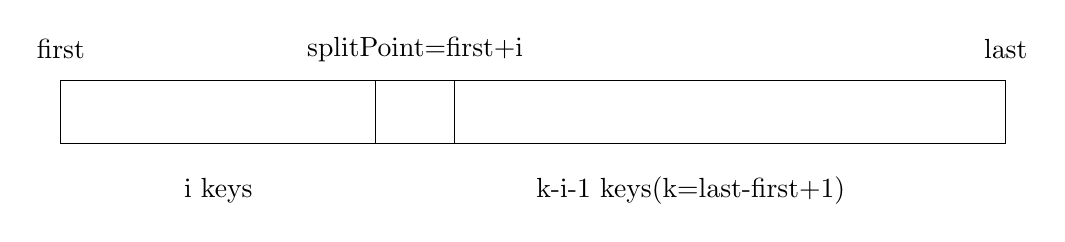
\begin{tikzpicture}[scale=1]
        \draw (0,0) rectangle (4,0.8);
        \draw (4,0) rectangle (5, 0.8);
        \draw (5,0) rectangle (12, 0.8);
        \node  at (0,1.2)[]  {first};
        \node  at (12,1.2)[]  {last};
        \node  at (4.5,1.2)[]  {splitPoint=first+i};
        \node  at (2,-0.6)[]  {i keys};
        \node  at (8,-0.6)[]  {k-i-1 keys(k=last-first+1)};
    \end{tikzpicture}
    \caption{快速排序的平均行为}
    \label{Fig:AverageBehaviorofQuicksort}
\end{figure*}

我们假设关键字是不同的,且所有关键字的排列都是等概率出现。令k是数组要排序范围
中的元素的个数,令A(k)是这个规模排序要做的平均关键字比较次数。假设下一次
Partition将pivot移动到了本次子范围的第i个位置(图\ref{Fig:AverageBehaviorofQuicksort}),
从0开始计数。Partion做了k-1次关键字比较,下一次要排序的子范围分别
有i个元素和k-1-i个元素。

在Partiition完成之后对于我们的分析是很重要的,子范围($first, \cdots, splitPoint-1$)
内没有两个关键字相互进行过比较,所以这个子范围内所有的排列依然是等概率的。同理
($splitPoint+1, \cdots, last$)也是一样。这一条有下面的递归。
\begin{displaymath}
\begin{aligned}
&A(n)=n-1+\sum_{i=0}^{n-1}\frac{1}{n}(A(i)+A(n-1-i)) \qquad  n\geq 2\\
&A(1)=A(0)=0
\end{aligned}
\end{displaymath}
检查和中的项以简化递归等式。形如A(n-1-i)的项run from A(n-1) down to A(0),所以
他们的和以A(i)的和同样。则我们可以丢弃A(0)项,得到
\begin{equation}\label{Equ:4_1}
A(n)=n-1+\frac{2}{n}\sum_{i=1}^{n-1}A(i)  \qquad  n\geq 1
\end{equation}
这是一个比我们前面看到的要复杂的递归等式,因为A(n)的值依赖于早先的值。我们可以
尝试使用一些技巧来解这个等式,或者我们可以猜一个解然后用归纳法证明这个解正确。
后一种技术特别适合递归算法。学习两种方法都是有益的,所以两种方法我们都会做。

为了猜A(n)的形式,让我们考虑一种快速排序工作的最好的情况。假设每次Partition执行
都将原来的范围分成两个等长的子范围。既然我们只是想从侧面猜测快速排序在平均情况
下有多块,我们将子范围的大小近似为n/2而不管这是不是一个整数。比较的次数描述为:
\begin{displaymath}
Q(n)\approx n+2Q(n/2)
\end{displaymath}
可以采用Master定理了(定理3.17):$b=2$,$c=2$,$E=1$,$f(n)=n^1$。因此
$Q(n)\in \Theta(n\log n)$。所以如果E[first]每次都接近split位置,则快速排序的
比较次数将在$\Theta(n\log n)$。这比$\Theta(n^2)$有显著的提高。但是如果关键字
所有的排列都是等概率出现的话,还会得到这么好的结果吗?我们将证明之。

\begin{theorem}
令A(n)由递归等式\ref{Equ:4_1}定义。则,对于$n \geq 1$,$A(n)\leq cn\ln n$,
c为常数。(注意:我们已经切换到自然数算法以简化证明中的一些计算。c的值将在证明中找到。)

{\textbf{\emph{证明}}}  证明归纳要排序的元素个数n。基本情况是n=1。
我们有$A(1)=0$,$c1\ln1=0$。

当$n>1$时,假设$A(i) \leq ci\ln(i)$,对于$1\leq i<n$,c是某个常数。通过
等式\ref{Equ:4_1}和归纳假设。
\begin{displaymath}
A(n)=n-1+\frac{2}{n}\sum_{i=1}^{n-1}A(i)\leq n-1+\frac{2}{n}\sum_{i=1}^{n-1}ci\ln(i)
\end{displaymath}
我们可以用积分划定边界(参看等式\ref{Equa:MonotonyFunctionA}):
\begin{displaymath}
\sum_{i=1}^{n-1}ci\ln(i)\leq c\int_1^nx\ln x dx
\end{displaymath}
使用\ref{Sec:Calculous}小节给出的等式\ref{Equa:1_15}有
\begin{displaymath}
\int_1^nx\ln x dx =\frac{1}{2}n^2\ln(n)-\frac{1}{4}n^2
\end{displaymath}
于是
\begin{displaymath}
\begin{aligned}
A(n)&\leq n-1 +\frac{2c}{n}\left(\frac{1}{2}n^2\ln(n)-\frac{1}{4}n^2\right)\\
&=cn\ln n+n(1-\frac{c}{2})-1
\end{aligned}
\end{displaymath}

为了满足$A(n)\leq cn\ln n$,第二项和第三项应该是负数或者0。对于$c\geq 2$的情况,
第二项小于等于0。所以我们可以令c=2并得出结论$A(n)\leq 2n\ln n$。
\end{theorem}

对于$c<2$的情况可以做类似的分析$A(n)>cn\ln n$。既然$\ln n\approx 0.693\lg n$,
我们有:

\begin{corollary}
在平均情况下,假设所有的输入的排列是等概率,快速排序(算法\ref{Algo:Quicksort})
做的平均比较次数对于大的n,近似为$1.386n\lg n$,n是输入集合的规模。
\end{corollary}

\subsubsection{更精确的平均行为*}
尽管我们已经建立了快速排序的平均行为,回到递归等式(等式4.1)依然是有益的,
尝试直接解这个等式可以得到更多的leading term。这一小节使用一些复杂的数学手段,
可以跳过本节不会影响学习的连续性。

由等式\ref{Equ:4_1}我们有

\begin{equation}\label{Equ:4_2}
A(n)=n-1+\frac{2}{n}\sum_{i-1}^{n-1}A(i)
\end{equation}

\begin{equation}\label{Equ:4_3}
A(n-1)=n-2+\frac{2}{n-1}\sum_{i-1}^{n-2}A(i)
\end{equation}

如果我们用\ref{Equ:4_2}减去\ref{Equ:4_3},大多数项都约掉了。既然和需要
乘上不同的因子,我们需要一个slightly more complicated bit of algebra。
非正式的,我们计算
\begin{displaymath}
n \times \mbox{式(\ref{Equ:4_2})} -(n-1) \times \mbox{式(\ref{Equ:4_3})}
\end{displaymath}
于是
\begin{displaymath}
\begin{aligned}
nA(n)-(n01)A(n01)&=n(n-1)+2\sum_{i-1}^{n-1}A(i)-(n-1)(n-2)-2\sum_{i-1}^{n-2}A(i)\\
&=2A(n-1)+2(n-1)
\end{aligned}
\end{displaymath}

有
\begin{displaymath}
\frac{A(n)}{n+1}=\frac{A(n-1)}{n}+\frac{2(n-1)}{n(n+1)}
\end{displaymath}
现在令
\begin{displaymath}
B(n)=\frac{A(n)}{n+1}
\end{displaymath}
对于B的递归等式是
\begin{displaymath}
B(n)=b(n-1)+\frac{2(n-1)}{n(n+1)} \qquad B(1)=0
\end{displaymath}
引用等式\ref{Equa:HarmonicSeries},我们过程留给读者验证
\begin{displaymath}
\begin{aligned}
B(n)&=\sum_{i=1}^n\frac{2(i-1)}{i(i+1)}=2\sum_{i=1}^n\frac{1}{i}-4\sum_{i=1}^n\frac{1}{i(i+1)}\\
&\approx 2(\ln n +0.577)-4n/(n+1)
\end{aligned}
\end{displaymath}
因此
\begin{displaymath}
A(n)\approx 1.386n\lg n -2.846n
\end{displaymath}

\subsubsection{空间使用}
第一眼看去似乎快速排序是一种in-place排序。但是不是。当算法在子范围上工作时,所有
其他范围的起至范围都要存放在frame stack中\footnote{译注:递归调用带来的},栈的规模
依赖于子范围的数量。当然就是依赖于n。在最坏情况下,Partition每次分隔一项;递归
的深度是n。因此最坏情况下的空间使用数量是$\Theta(n)$。下面描述的一个算法的改进
能显著的减少栈的尺寸。

\subsection{基本快速排序算法的改进}\label{Sec:ImprovementsOntheBasicQuicksortAlgorithm}
\subsubsection{选择枢轴}
我们已经看到如果Partition使用的pivot能分成两个基本一样大小的段时,快速排序
就会很好。(它的位置是Partition返回的splitPoint。)选择E[first]作为pivot时可能
导致快速排序很糟糕,而本来这时排序会是很简单的,比如当数组已经是有序的情况。有
许多其他的选择pivot的策略。一种是选一个first和last之间的随机整数q,令pivot=E[q].key。
另一个是另pivot是E[first], E[(first+last)/2], E[last]的中间一个。(两种情况下,
在Partition之前E[first]元素都将先和pivot元素交换。)两种策略都需要在选择pivot
时做一点额外工作,但是他们会减少快速排序程序的平均运行时间。

\subsubsection{可选的Partiton策略}
文中展示的Partition版本在平均情况下做最少的元素移动,与其他partitioning策略
比较。这个子例程比较清晰,and coding these in-line would save some overhead;
但是有些编译器可以自动做这种优化。其他优化考虑在本章后面的Notes和References中
提及。在练习中有一个可选版本,连续中的版本易于理解和编程,但是稍慢。

\subsubsection{小集合排序}
实际应用中快速排序对于小的集合效果不佳,因为有太多的过程调用。但是,快速排序
算法对于大到n的规模也会分解成小的子集合再递归排序他们。因此,当子集合小的
一定程度时,算法就变的低效率了。这个问题可以通过下面的方法来补偿,选择一个
小的smallSize,当集合的大小小于或等于smallSize的时候采用简单非递归的排序,在
改进过的算法中调用了smallSort。(此时插入排序是个不错的选择。)

\begin{lstlisting}[language={Java}, keywordstyle=\color{blue!70}, commentstyle=\color{red!50!green!50!blue!50}]
quickSort(E, first, last)
{
    if( last -first)>smallsize)
    {
        pivotElement=E[first];
        pivot=pivotElement.Key;
        int splitPoint=partition(E, pivot, first, last);
        E[splitPoint]= pivotElement;
        quickSort(E, first, splitPoint-1);
        quickSort(E, splitPoint+1, last);
    }
    else
        smallSort(E, first, last);
}
\end{lstlisting}

这个方案的一个变体是跳过调用smallSort。则当快速排序退出时,数组
不是有序的,但是所有的元素都只需要移动小于smallSize的位置就能到
达它正确(排序好的)的位置。(为什么?)因此作为后处理,进行一次
插入排序将是非常有效的,而且不会像前面那个版本中的smallSort调用
做很多相同的比较。

smallSize该取多大呢?最好的选择依赖于算法具体的实现(也就是使用
的计算机,以及程序的细节),因而我们可以在overhead和比较之间做
一下取舍。10是一个合理的值。

\subsubsection{堆栈空间优化}
我们观察到Quicksort的递归调用深度可能很深,最坏情况下可能达到n(在Partition每次
只分解一个元素的时候)。许多pushing和poping的都是不必要的。Partition之后,程序
开始排序子范围$E[first], \cdots, E[solitPoint-1]$;之后它必须排序
$E[splitPoint+1], \cdots, E[last]$。

第二个递归调用是过程的最后一句话,所以可以用我们前面在插入排序中用于shiftVac的方式
将第二个递归转换成迭代。第一个递归依然在那里,所以只是部分的消除了递归。

尽管只有过程中只有一个递归调用了,我们仍然要关心递归深度。当每次递归调用只能比前
一次稍微小一点时,递归深度就是个问题。所以我们使用的第二个技巧是避免递归在大的
子范围做递归。通过保证每次递归调用在接近它的“父”递归调用一半的子范围上,
递归深度保证维持在lgn。两个ideal合并在下面的版本中,“TRO”表示“尾递归优化(tail
recursion optimization)”。想法是在每次partition之后,下一次递归将在小的那个
子范围上,大的子范围将直接用while循环处理。

\begin{lstlisting}[language={Java}, keywordstyle=\color{blue!70}, commentstyle=\color{red!50!green!50!blue!50}]
quickSortTRO(E, first, last)
{
    int first1, last1, first2, last2;

    first2= first; last2= last;
    while( last2- first2 >=1)
    {
        pivotElement = E[first2];
        pivot= pivotElement.Key;
        int splitPoint=partition(E, pivot, first2, last2);
        E[splitPoint]= pivotElement;
        if(splitPoint<= (first2+ last2)/2)
        {
            first1=first2; last1=splitPoint -1;
            first2= splitPoint+1; last2 =last2;
        }
        else
        {
            first1= splitPoint +1; last1= last2;
            first2= first2;  last2 =splitPoint-1;
        }
    }
    return;
}
\end{lstlisting}

\subsubsection{结合使用这些改进手段}
前面我们独立的讨论几种修改方法,但是他们可以协调的组合在一个程序中。

\subsubsection{Remarks}
实际中,快速排序程序对大的n平均而言运行的很快,是广泛使用的一种排序方法。但是
在最坏情况下,快速排序很糟糕。类似插入排序(参看\ref{Sec:InsertSort}小节),
Maxsort和冒泡排序(练习4.1和4.2),快速排序最坏情况是$\Theta(n^2)$,但是与其他
不同,快速排序平均行为在$\Theta(n\log n)$。有排序算法最坏情况能在
$\Theta(n\log n)$吗,或者我们可以建立最坏情况的底限就是$\Theta(n^2)$。让我们
再次检查通用的技术,看看如何改进最坏情况下的行为。

\section{归并有序序列}
在这一节中我们回顾一下下面问题的直接解决方案:给定两个升序序列A和B,归并两者得到
一个新的序列C。归并有序的子序列是归并排序的关键策略。归并有序子序列同样有许多的
方法,在练习中有提及。衡量归并算法的度量是关键字比较的次数。

令k和m是分别是A和B元素的数量。令n=k+m是“问题的规模”。假设A和B都不是空的,我们可以
立即决定C的第一个元素:就是A和B的第一个元素中小的那个。C剩下的部分呢?假设A的
第一个元素是比B的小。则C剩下的部分肯定是A除第一个元素外所有的元素和B所有元素的
归并。这只是我们开始那个问题的一个小一点的版本。如果C的第一个元素是来自B的,问题
是对称的。两种情况下剩下问题的规模(构造C剩下的部分)都是n-1。
Method99(\ref{Sec:HintsForRecursionMethod99}小节)。

如果我们假定我们仅需要归并规模是100的问题,而且我们可以调用merge99来归并规模
是99的问题,则问题就解决了。伪代码如下:
\begin{lstlisting}[language={Java},keywordstyle=\color{blue!70}, commentstyle=\color{red!50!green!50!blue!50}]
merge(A,B,C)
    if(A is null)
        rest of C =rest of B;
    else
        if(B is null)
            rst of C =rest of A;
        else
            if (first of A<= first of B)
                first of C= first of A;
                merge99(rest of A, b, rest of C);
            else
                first of C= first of B;
                merge99(A, rest of B,rest of C);
    return;
\end{lstlisting}

现在只需要将merge99换成merge就是一个递归解决方案了。

一旦有一个解决方案,我们就可以想办法将它变成一个迭代解决方案。理想的情况是对于
所有的连续数据结构可用,但是在不指明的情况下,我们的算法仅限于数组。我们在
迭代每次开始的时候引入3个索引来跟踪“rest of A”,“reat of B”和“rest of C”。
(这些索引在递归版本中是参数。)

\begin{algorithm}\label{Algo:Merge}
归并

{\textbf{\emph{输入:}}}数组A有k个元素,B有m个元素,两个数组
都是升序的。

{\textbf{\emph{输出:}}}C,一个数组包含n=k+m个来自A和B的元素,
同样以升序排列。C是传入的,算法填充它。
\end{algorithm}
\begin{lstlisting}[language={Java},keywordstyle=\color{blue!70}, commentstyle=\color{red!50!green!50!blue!50}]
void merge(Element[] A, int k, Element[] B, int m, Element[] C)
{
    int n=k+m;
    int indexA=0, indexB=0, indexC=0;
    // `indexA是rest of A最开始的位置,B和C类似。`
    while(indexA<k && indexB<M)
    {
        if(A[indexA].key<=B[indexB].key)
        {
            C[indexC]=A[indexA];
            indexA++;
            indexC++;
        }
        else
        {
            C[indexC]B[indexB];
            indexB++;
            indexC++;
        }
    }
    if(indexA>=k)
        `Copy B[indexB,…,m-1] to C[indexC,…,n-1].`
    else
        `Copy A[indexA,…,k-1] to C[indexC,…,n-1].`
}
\end{lstlisting}

\subsection{最坏情况}
只要A和B中的关键字有一次比较,至少有一个元素移动到C,而且不会在检查这个元素了。
在最后一次比较之后,至少有两个元素--两个参加比较的--还没有进入C。小的那个马上
移动进去了,但是现在C至多有n-1个元素,而再没有比较了。剩下的工作就是将某个数组
剩下的元素移动到C不做任何比较。所以最多有n-1次比较,最坏情况下所有的n-1次比较,
即A[k-1]和B[m-1]刚好是C的最后两个元素时。

\subsection{归并的优化}
下面我们将演示,当k=m=n/2时在基于比较的算法的最坏情况下,算法\ref{Algo:Merge}是
最优的。就是说,对于任何基于比较的算法为了在k=m=n/2的时候要想所有的输入都
正确,至少存在某些输入必须要做n-1次比较。(这并不是说,对于某些特定的输入
有算法要比算法\ref{Algo:Merge}要好。)考虑完k=m=n/2之后,我们再看看k和m的
其他关系。

\begin{theorem}\label{Theorem:4_4}
所有通过比较关键字归并两个含有k=m=n/2元素有序数组的算法,在最坏情况下至少要
做n-1次比较。

{\textbf{\emph{证明}}}  假设我们给出任意归并算法。令$a_i$和$b_i$分别是A和B
的第i个元素。我们可以选出一组keys,使得算法必须比较$a_i$到
$b_i$($0\leq i<m$),以及$a_i$到$b_{i+1}$(对于所有$0\leq i<m-1$)。
特定的,按如下方式选出key,即任何时候当算法比较$a_i$和$b_i$,如果$i<j$,
则结果是$a_i<b_j$,如果$i\geq j$,则结果是$b_j<a_i$。选择如下key
\begin{equation}\label{Equ:4_4}
b_0<a_0<b_1<a_1<\cdots b_i<a_i<b_{i+1}<\cdots b_{m-1}<a_{m-1}
\end{equation}
将满足条件。但是,对于某些i,算法永远不比较$a_i$和$b_i$,则等式\ref{Equ:4_4}
的顺序选出keys,除了没有$a_i<b_j$,也将满足条件,但是算法不能得到正确的顺序。

类似的,如果对于某些i,算法从不比较$a_i$和$b_{i+1}$,等式\ref{Equ:4_4}的排列,
除了$b_{i+1}<a_i$,其他的关系都能由比较得到,但是算法还是不能决定正确的顺序。
\footnote{译注:这里的证明过程实际上就是构造了一个输入序列满足等式\ref{Equ:4_4},即
最坏情况,然后证明,如果少于n-1次比较将不能得到正确的顺序。}
\end{theorem}

我们能一般化这个结论吗?假设k和m是不相等的(就像我们在归并排序中遇到的)?

\begin{corollary}\label{corollary:4_5}
两个有序序列分别包含k和m个元素,k和m相差1,n=k+m,任意通过比较归并
两个有序序列的算法,将至少做n-1次比较。

{\textbf{\emph{证明}}} 证明过程和\ref{Theorem:4_4}类似,除了没有$a_{m-1}$
\end{corollary}

我们能更进一步的一般化我们的结论吗?如果我们能找到一种极端情况的行为,检查
另一个极端通常是一个好主意。这里,第一个“极端”是k=m,所以另一个极端是k和m
差的尽可能的大。让我们看另一种极端情况,k=1,m非常大,n=m+1。我们可以设想
算法至少使用$\lceil\lg(m+1)\rceil$次比较(为什么?\footnote{译注:相当于做二分查找})
于是显然n-1不是这种情况的底限。k=1的情况可以一般化为k远小于n的情况
(练习4.24)。因此,定理\ref{Theorem:4_4}和推论\ref{corollary:4_5}的底限
不能扩展到所有k和m的组合。等多可能性的情况在读完
\ref{Sec:LowerBoundsForSortingByComparisonOfKeys}节后,参看练习4.33。

\subsection{空间使用}\label{Sec:MergeSpaceUsage}
因为所有的元素都要拷贝到C,从算法\ref{Algo:Merge}看出归并总数是n的条目
需要2n个元素的空间。然而有些情况下,需要额外空间的数量可能减少。比如,
序列是链表。则在合并完成之后A,B就不需要了,A和B的元素重新组成了C。

\begin{figure*}[!t]
    \centering
    \begin{tikzpicture}[scale=1]
        \draw[] (0,0) rectangle (6,1);
        \draw[] (9,0) rectangle (12,1);
        \draw[] (0,-0.5) node[right] {0};
        \draw[] (6,-0.5) node[left] {n+m-1};
        \draw[] (3,-1) node {Merged lists};
        \draw[] (9,-0.5) node[right] {0};
        \draw[] (12,-0.5) node[left] {m-1};
        \draw[] (10.5,-1) node {B};
        \draw[] (10.5,0.5) node {Empty};
        \foreach \x in {0,...,5, 0.5,...,4.5}
            \draw (\x, 1) -- (\x +1 , 0);
        \draw (0, 0.5) -- (0.5 , 0);
        \draw (5.5, 1) -- (6 , 0.5);
        \foreach \x in {1,...,6, 1.5,...,5.5 }
            \draw (\x, 1) -- (\x -1 , 0);
        \draw (0.5, 1) -- (0 , 0.5);
        \draw (5.5, 1) -- (6 , 0.5);
        \draw[] (0,1.5) node[right] {完成};

        \draw[] (0,4) rectangle (6,5);
        \draw[] (9,4) rectangle (12,5);
        \draw[] (2,4) rectangle (3,5);
        \draw[] (9,4) rectangle (10,5);
        \draw[] (0,3.5) node[right] {0};
        \draw[] (6,3.5) node[left] {n+m-1};
        \draw[] (4,3.5) node {n-1};
        \draw[] (0,3) node[right] {A中剩下的keys};
        \draw[] (6,3) node[left] {归并过的keys};
        \draw[] (9,3.5) node[right] {0};
        \draw[] (12,3.5) node[left] {m-1};
        \draw[] (10.5,3) node {B};
        \draw[] (0,5.5) node[right] {归并中};
        \foreach \x in {9}
            \draw (\x, 5) -- (\x +1 , 4);
        \draw (9, 4.5) -- (9.5 , 4);
        \draw (9.5, 5) -- (10,4.5);
        \foreach \x in {1, 2, 1.5 }
            \draw (\x, 5) -- (\x -1 , 4);
        \draw (0.5, 5) -- (0 , 4.5);
        \draw (2, 4.5) -- (1.5,4);

        \foreach \x in {3,...,5, 3.5,...,4.5}
            \draw (\x, 5) -- (\x +1 , 4);
        \draw (3, 4.5) -- (3.5 , 4);
        \draw (5.5, 5) -- (6 , 4.5);
        \foreach \x in {4,...,6, 4.5,...,5.5 }
            \draw (\x, 5) -- (\x -1 , 4);
        \draw (3.5, 5) -- (3 , 4.5);
        \draw (6, 4.5) -- (5.5 , 4);

        \draw[] (0,7) rectangle (6,8);
        \draw[] (9,7) rectangle (12,8);
        \draw[] (4,7) rectangle (6,8);
        \draw[] (0,6.5) node[right] {0};
        \draw[] (6,6.5) node[left] {n+m-1};
        \draw[] (4,6.5) node {n-1};
        \draw[] (3,6) node {A};
        \draw[] (9,6.5) node[right] {0};
        \draw[] (12,6.5) node[left] {m-1};
        \draw[] (10.5,6) node {B};
        \draw[] (0,8.5) node[right] {归并之前};
        \draw[] (5,7.5) node {Empty};
        \foreach \x in {1,...,4, 1.5,...,3.5 }
            \draw (\x, 8) -- (\x -1 , 7);
        \draw (0.5, 8) -- (0 , 7.5);
        \draw (4, 7.5) -- (3.5,7);
        \foreach \x in {9, 9.5, 10, 10.5, 11}
            \draw (\x, 8) -- (\x +1 , 7);
        \draw (9, 7.5) -- (9.5 , 7);
        \draw (11.5, 8) -- (12,7.5);
    \end{tikzpicture}
    \caption{归并使用Overlapping数组}
    \label{Fig:Overlapping arrays for Merge}
\end{figure*}

假定输入的序列存储在数组中,且有$k\geq m$。如果A有足够的空间来放$n=k+m$
个元素,则只需要A中的额外m个元素就可以了。简单的将C以A来标识,然后从A和B的
右端开始做归并(大关键字的一端),如图\ref{Fig:Overlapping arrays for Merge}
所示。最先移动到“C”$m$个条目将填充A额外的空间。从那时开始,A中的空位
被使用了。在所有条目被归并完之前,在以归并完成的位置和A剩下的条目之间
总会有一个gap(也就是说,有一些空位)。显然如果使用这种节省空间存储方式,
归并算法的最后一行(\textbf{else} Copy A[indexA,…,k-1] to C[indexC,…,n-1])
可以被消除,因为:如果B比A先空,A中剩下的条目就在他们正确的位置,不需要移动。

不管C有没有overlap到输入数组,当$k=m=n/2$时,归并算法使用的额外空间在$\Theta(n)$

\section{归并排序}\label{Sec:Mergesort}

\begin{figure*}[!t]
    \centering
    \begin{tikzpicture}[scale=1]
        \draw (0,0) rectangle (12,1);
        \draw[] (6,0.5) node {Sorted};

        \draw (0,3) rectangle (12, 4);
        \draw[] (3,3.5) node {Sorted};
        \draw[] (9,3.5) node {Sorted};
        \draw[] (6,4)--(6,3);
        \node  at (6,2)[]  {Merge};
        \draw[->] (3,2.8)--(4,1.2);
        \draw[->] (9,2.8)--(8,1.2);

        \draw (0,6) rectangle (12, 7);
        \node  at (0,7.2)[]  {first};
        \node  at (12,7.2)[]  {last};
        \draw[] (6,6)--(6,7);
        \node  at (6,8)[]  {$\lfloor(first+last)/2\rfloor$};
        \node  at (3,5)[]  {递归调用归并排序};
        \node  at (9,5)[]  {递归调用归并排序};
        \draw[->] (1.5,5.8)--(1.5,4.2);
        \draw[->] (10.5,5.8)--(10.5,4.2);
    \end{tikzpicture}
    \caption{归并排序策略}
    \label{Fig:MergesortStrategy}
\end{figure*}

Quicksort的问题是Partition不能总是将数组分成两个相等的部分。归并排序将
数组分成两相等的部分,再分别排序(当然是递归的)。之后它归并两个已经
有序的部分(参看图\ref{Fig:MergesortStrategy})。因此,使用
\ref{Sec:DividAndConquer}节的分而治之技术,“分”仅仅是计算
子范围的中间索引没有任何关键字比较;“和”是归并。

我们假定归并改成合并数组两个相邻的子范围,将合并之后的数组放回原来的
空间。它的参数现在是E、要合并的子范围的索引是first、mid、last;排序的
子序列是$E[first],\cdots ,E[mid]$和$E[mid+1],\cdots ,E[last]$,最后
完成排序的序列是$E[first],\cdots ,E[last]$。这样修改之后,merge子例程
还是需要分配额外的空间。其中一些主题在\ref{Sec:MergeSpaceUsage}小节
中讨论过了。

\begin{algorithm}
归并排序

{\textbf{\emph{输入:}}}数组E索引first,last,E[i]($first\leq i \leq last$ )

{\textbf{\emph{输出:}}}E[first]…E[last] 是已经有序的元素。
\end{algorithm}

我们发现学生经常将Merge和Mergesort搞混。记住归并排序Mergesort是一种
排序算法。它用于将\emph{一个}杂乱的数组排序。归并Merge用于将\emph{两个}
已经有序的数组合成一个有序的数组。

\begin{lstlisting}[language={Java},keywordstyle=\color{blue!70}, commentstyle=\color{red!50!green!50!blue!50}]
void mergeSort(Element[] E, int first, int last)
{
    if(first<last)
    {
        int mid=(first+last)/2;
        mergeSort(E,first,mid);
        mergeSort(E,mid+1, last);
        merge(E,first,mid,last);
    }
}
\end{lstlisting}

\subsubsection{归并分析}
首先找到最坏情况下Mergesort关键字比较的渐进阶。我们定义问题的规模
$n=last-first+1$,要排序的元素个数。递归排序最坏情况的递归等式是
\begin{equation}\label{Equ:4_5}
\begin{aligned}
W(n)&=W(\lfloor n/2\rfloor)+W(\lceil n/2\rceil)+n-1\\
W(1)&=0
\end{aligned}
\end{equation}
Master定理马上告诉我们$W(n)\in \Theta(n\log n)$。所以终于,我们有了一个
最坏情况下在$\Theta(n\log n)$的排序算法。我们在这里就不开辟新的一小节
来分析平均复杂性,我们将这个问题推迟到我们发展出更通用的
定理\ref{Theorem::LowerBoundOfSort}之后再讨论,定理\ref{Theorem::LowerBoundOfSort}
关注平均行为,就在后面的\ref{Sec:LowerBoundsForSortingByComparisonOfKeys}
节讨论。

归并排序一个可能的缺点是它需要辅助空间。因为归并需要的额外空间在$\Theta(n)$,
归并排序不是一个in-place排序。

\subsubsection{*更精确的归并排序分析}
根据下一节(\ref{Sec:LowerBoundsForSortingByComparisonOfKeys})求出的底限,
有时候需要得到最坏情况下比较次数的的精确值。我们可以看出Mergesort非常
接近低限。读者可以跳过本小节的细节直接去看主要结论,定理\ref{Theorem:4_6}。

\begin{figure*}[!t]
    \centering
    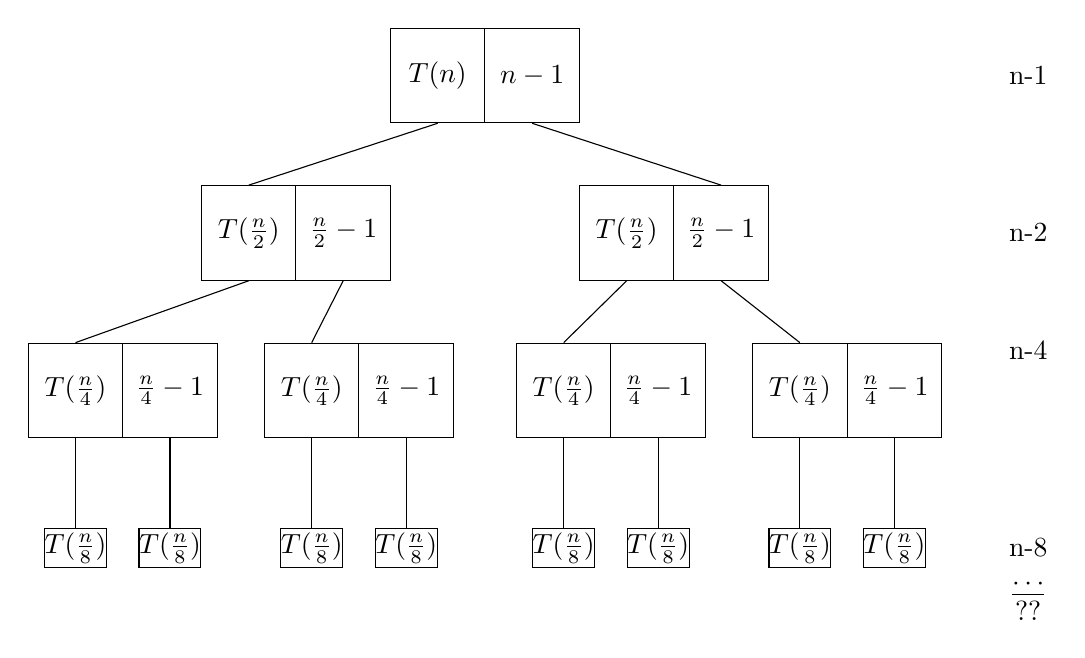
\begin{tikzpicture}[scale=1,place/.style={rectangle,draw, fill=white,inner sep=0pt,minimum size=12mm},
                            do/.style={rectangle,draw, fill=white,inner sep=0pt,minimum size=5mm}]
    \node (P6)  at (0,0) [place] {$T(n)$};
    \node (P5)  at (1.2,0) [place] {$n-1$};
    \node (P4)  at (-2.4,-2) [place] {$T(\frac{n}{2})$};
    \node (P3)  at (-1.2,-2) [place] {$\frac{n}{2}-1$};
    \node (P2)  at (2.4,-2) [place] {$T(\frac{n}{2})$};
    \node (P1)  at (3.6,-2) [place] {$\frac{n}{2}-1$};

    \node (P41)  at (-4.6,-4) [place] {$T(\frac{n}{4})$};
    \node (P31)  at (-3.4,-4) [place] {$\frac{n}{4}-1$};
    \node (P21)  at (-1.6,-4) [place] {$T(\frac{n}{4})$};
    \node (P11)  at (-0.4,-4) [place] {$\frac{n}{4}-1$};
    \node (P42)  at (1.6,-4) [place] {$T(\frac{n}{4})$};
    \node (P32)  at (2.8,-4) [place] {$\frac{n}{4}-1$};
    \node (P22)  at (4.6,-4) [place] {$T(\frac{n}{4})$};
    \node (P12)  at (5.8,-4) [place] {$\frac{n}{4}-1$};

    \node (P83)  at (-4.6,-6) [do] {$T(\frac{n}{8})$};
    \node (P73)  at (-3.4,-6) [do] {$T(\frac{n}{8})$};
    \node (P63)  at (-1.6,-6) [do] {$T(\frac{n}{8})$};
    \node (P53)  at (-0.4,-6) [do] {$T(\frac{n}{8})$};
    \node (P43)  at (1.6,-6) [do] {$T(\frac{n}{8})$};
    \node (P33)  at (2.8,-6) [do] {$T(\frac{n}{8})$};
    \node (P23)  at (4.6,-6) [do] {$T(\frac{n}{8})$};
    \node (P13)  at (5.8,-6) [do] {$T(\frac{n}{8})$};

    \draw (P6.south)--(P4.north);
    \draw (P5.south)--(P1.north);
    \draw (P4.south)--(P41.north);
    \draw (P3.south)--(P21.north);
    \draw (P2.south)--(P42.north);
    \draw (P1.south)--(P22.north);

    \draw (P41.south)--(P83.north);
    \draw (P31.south)--(P73.north);
    \draw (P21.south)--(P63.north);
    \draw (P11.south)--(P53.north);
    \draw (P42.south)--(P43.north);
    \draw (P32.south)--(P33.north);
    \draw (P22.south)--(P23.north);
    \draw (P12.south)--(P13.north);

    \node (Px1)  at (7.5,0)  {n-1};
    \node (Px2)  at (7.5,-2)  {n-2};
    \node (Px3)  at (7.5,-3.5)  {n-4};
    \node (Px5)  at (7.5,-6)  {n-8};
    \node (Px4)  at (7.5,-6.5) {\underline{$\cdots$}};
    \node (Px6)  at (7.5,-6.8)  {??};
    \end{tikzpicture}
    \caption{归并排序的递归树。}
    \label{Fig:RecursionTreeForMergesort}
\end{figure*}

在等式\ref{Equ:4_5}的递归树(参看图\ref{Fig:RecursionTreeForMergesort})
中,我们观察到深度为$d$的节点s的非递归消耗的和是$n-2^d$(对于所有同
深度节点,不包含基本情况。)。我们可以得出所有的基本情况在($W(1)=0$)在
深度$\lceil \lg(n+1)\rceil -1$或$\lceil\lg(n+1) \rceil$。恰好有n个基本情
况节点。令最大深度为D,(也就是$D=\lceil\lg(n+1) \rceil$),令B是深度为
$D-1$时基本情况的的数目。则在深度$D$有$n-B$个基本情况(而且在深度D没有
其他的节点)。在深度$D-1$的每一个非基本情况节点都有两个孩子,于是在深度
$D-1$有$(n-B)/2$个非基本情况节点。使用这些信息,我们计算最后几层深度的
非递归消耗如下:
\begin{enumerate}
\item 深度$D-2$有$2^{D-2}$节点,其中没有一个基本情况节点。这一层的非递归
    消耗是$n-2^{D-2}$。
\item 深度$D-1$有$(n-B)/2$个非基本情况。每一个非基本情况节点的问题规模是2
(其消耗是1),于是这一层的非递归消耗是$(n-B)/2$。
\item 深度$D$有$n-B$个基本情况,消耗是0。
\end{enumerate}
你可以验证$B=2^D-n$(练习4.29)。因此

\begin{equation}\label{Equ:4_6}
\begin{aligned}
W(n)&=\sum_{d=0}^{D-2}(n-2^d)+(n-B)/2\\
&=n(D-1)-2^{D-1}+1+(n-B)/2
&=nD-2^D+1
\end{aligned}
\end{equation}
因为D是通过取整运算到一个整数的,且在指数项中出现,很难给出等式\ref{Equ:4_6}
的行为在2的指数函数中的那个范围。我们证明下面的定理,它从指数中移除取整函数。

\begin{theorem}\label{Theorem:4_6}
最坏情况下归并排序的比较次数在$\lceil n\lg(n)-n+1 \rceil$和
$\lceil n\lg(n)-0.914n \rceil$之间

\noindent {\textbf{\emph{证明}}} 如果我们定义了$\alpha = 2^D/n$,则$1\leq \alpha <2$,
且在等式\ref{Equ:4_6}中,将D替换成$(\lg(n))+lg(\alpha)$。这将得到
$W(n)=n\lg(n)- (\alpha - \lg\alpha)n +1$。$(\alpha -\lg \alpha)$的最小值约
是0.914(参见练习4.30),最大值在1之内。
\end{theorem}

归并排序在最坏情况下约比快速排序在平均情况下少30\%的比较次数。但是,平均情况下
归并排序比快速排序移动元素的次数要多,所以有些时候它并不比快速排序要快(参看
练习4.21和练习4.27)。

\section{基于比较的排序的底限}\label{Sec:LowerBoundsForSortingByComparisonOfKeys}
插入排序和快速排序做的关键字比较次数在最坏情况下在$\Theta(n^2)$。我们能用
归并排序加以改进,使得最坏情况在$\Theta(n\log n)$。我们能做的更好吗?

在本节中我们得到任何通过比较关键字来排序算法在最坏情况下和平均情况下必须做的比较
次数的底限。这个结果告诉我们我们可以停止寻找更好的算法了。为了得到底限,我们假设
待排序数组中的关键字是互不相同的。

\subsection{排序算法的判定树}\label{Sec:DecisionTreesForSortingAlgorithms}
\begin{figure*}[!t]
    \centering
    \begin{tikzpicture}[scale=0.8,place/.style={circle,draw, fill=white,inner sep=0pt,minimum size=8mm}
        ,ex/.style={ellipse,draw, fill=white,inner sep=0pt,minimum size=8mm}]
    \node (x3)  at (3.5,0) [ex] {$x_1,x_3,x_2$};
    \node (x4)  at (6.5,0) [ex] {$x_3,x_1,x_2$};
    \node (x7)  at (11.5,0) [ex] {$x_2,x_3,x_1$};
    \node (x8)  at (14.5,0) [ex] {$x_3,x_2,x_1$};
    \node (x21)  at (1,1.5) [ex] {$x_1,x_2,x_3$};
    \node (x22)  at (5,1.5) [place] {1:3};
    \node (x23)  at (9,1.5) [ex] {$x_2,x_1,x_3$};
    \node (x24)  at (13,1.5) [place] {2:3};
    \node (x31)  at (3,3) [place] {2:3};
    \node (x32)  at (11,3) [place] {1:3};
    \node (x41)  at (7,4.5) [place] {1:2};
    \draw [thick] (x41) -- (x31);
    \draw [thick] (x41) -- (x32);
    \draw [thick] (x31) -- (x21);
    \draw [thick] (x31) -- (x22);
    \draw [thick] (x32) -- (x23);
    \draw [thick] (x32) -- (x24);
    \draw [thick] (x22) -- (x3);
    \draw [thick] (x22) -- (x4);
    \draw [thick] (x24) -- (x7);
    \draw [thick] (x24) -- (x8);
    \end{tikzpicture}
    \caption{排序算法的决策树,n=3}
    \label{Fig:DecsisionTreeForSorting}
\end{figure*}

令n是固定值,假设关键字是$x_1,x_2,\cdots, x_n$。我们将每一个算法和一个
正整数$n$想关联,一颗(二叉树)决策树描述的比较关键字的序列就是算法对
任意输入规模n的行为。令Sort是任意通过比较关键字排序的算法。每一次比较
有两个分支(因为关键字是互不相同的),我们假设Sort有一个输出指令以输出
重新排列之后的关键字s。Sort的决策树由一棵树归纳定义,树由每一个比较和
每一个输出指令的构成。每一个和树关联的输出指令是一个节点,节点表示一个
关键字s的重排。每一个和树关联的比较($x_i$和$x_j$)是一颗树,其根是标
记了$(i:j)$的节点,其左子树中所有的比较和输出都是当$x_i<x_j$时的情况,
其右子树中所有的比较和输出都是当$x_i>x_j$的情况。Sort的决策树是第一次
比较指令执行完之后的树。图\ref{Fig:DecsisionTreeForSorting}展示了一个
$n=3$的决策树的例子。

特定输入Sort的行为对应着从决策树的根沿着一条path到叶子。决策树必须
有至少$n!$个叶子,因为对于$n$个关键字有$n!$种排列。既然每一个输入的
的唯一路径仅依赖于输入中关键字的顺序(order),而不依赖于他们具体的值,
实际执行Sort中,$n!$个叶子中的每一个都可以从根到达。我们将假设树中从
没有被走过的路径将被移除。我们还假设仅有一个孩子的比较节点将被移除并
被取代成孩子,这种“修剪”将一直持续到所有的internal节点的度都成2。
修剪过的树表示的算法至少和原来的一样有效率,所以我们用恰好有$n!$个叶子
的决策树得出的底限,和用所有的internal节点度都是2的决策树得出的底限将
是对所有以比较关键字排序的算法都有效。到现在为止,我们假设Sort以这样一
颗树来描述。

对于特定输入来说Sort做比较的次数就是这套输入所有的路径上internal节点的
数量。因此最坏情况下比较的次数就是最长的路径上internal节点的数量,也
就是树的高度。比较的平均次数是所有从根到叶子路径的平均长度。(例如,对于
$n=3$,图\ref{Fig:DecsisionTreeForSorting}中描述的算法在最坏情况下做
3次比较,平均做$2\frac{2}{3}$次比较。)

\subsection{最坏情况的底限}\label{Sec:LowerBoundOfWorstCase}
为了得到通过比较排序的最坏情况的底限,我们先得到确定叶子数量后高度
的底限,因为我们知道的关于决策树唯一的数量信息是叶子的数量。

\begin{lemma}\label{Lemma:4_7}
令$L$是二叉树中叶子的数量,令$h$是二叉树的高。则$L\leq 2^h$。

\noindent{\textbf{\emph{证明: }}}简单直接的归纳h即可。
\end{lemma}

\begin{lemma}\label{Lemma:4_8}
令$L$和$h$如\ref{Lemma:4_7}的定义。则$h\geq \lceil\lg L\rceil$。

\noindent{\textbf{\emph{证明: }}}将\ref{Lemma:4_7}中不等式的两边同时取对数得到
$\lg L \leq h$。既然$h$是整数,则$h\geq \lceil \lg L\rceil$。
\end{lemma}

\begin{lemma}\label{Lemma:4_9}
对于给定的$n$,通过比较关键字来排序的任意算法的决策树的高至少是
$\lceil\lg n!\rceil$。

\noindent{\textbf{\emph{证明: }}}将\ref{Lemma:4_8}中,取$L= n!$。
\end{lemma}

所以,最坏情况下比较的次数至少是$\lceil\lg n!\rceil$。迄今为止我们最好
的sort是归并排序,但是$\lceil\lg n!\rceil$和$n\lg n$和有多接近?为了寻找
答案,我们需要将$\lg n!$变成一种更方便的形式,并找打它的底限。有好几种
变化方法。可能最简单的,但是不是非常精确的如下
\begin{displaymath}
n! \geq n(n-1)\cdots (\lceil n/2 \rceil) \geq \left( \frac{n}{2} \right)^{\frac{n}{2}}
\end{displaymath}
于是
\begin{displaymath}
\lg n! \geq \frac{n}{2}\lg\frac{n}{2}
\end{displaymath}
这是在$\Theta(n\log n)$。因此我们已经看到归并排序有最优的渐进阶。为了
获得接近的底限,我们使用事实
\begin{displaymath}
\lg n! = \sum_{j=1}^n \lg (j)
\end{displaymath}
使用等式\ref{Equa:1_18}我们得到
\begin{displaymath}
\lg n! \geq n\lg n - (\lg e)n
\end{displaymath}
这里$e$表示自然对数,$\lg(e)$约是1.443。因此决策树的高度至少是
$\lceil n\lg n -1.443n \rceil$。

\begin{theorem}\label{Theorem:4_10}
任何用比较来排序关键字的算法,在最坏情况下排序n个元素,至少要做
$\lceil\lg n!\rceil$,约$\lceil n\lg n -1.443n \rceil$次比较。
\end{theorem}

So,归并排序是非常接近最优的。在归并排序的精确行为和底限之间依然
有些偏差。考虑$n=5$的情况。插入排序在最坏情况下做10次比较,归并
排序是8,但是底限是$\lceil\lg n! \rceil=\lceil \lg 120 \rceil=7$。
是因为我们求得底限不够精确,还是我们可以让归并排序做的更好呢?我们
鼓励你尝试去找到一种只用7次比较就能排序5个元素的方法(练习4.32)。


\subsection{平均行为的底限}\label{Sec:LowerBoundOfAverageBehavior}

\begin{figure*}[!t]
    \centering
    \subfloat[给出$L$的2-tree]{
        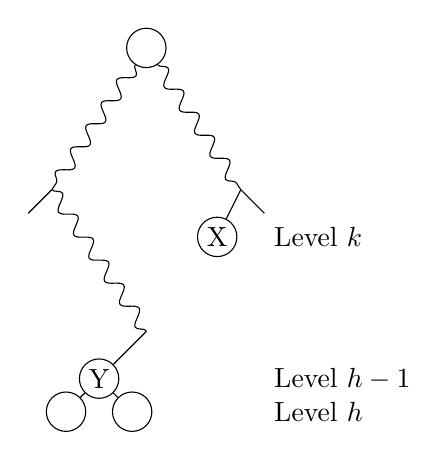
\begin{tikzpicture}[scale=0.6,place/.style={circle,draw, fill=white,inner sep=0pt,minimum size=5mm}]
            \node (x31)  at (1,5) [place] { };
            \draw [decorate,decoration=snake] (x31) -- (-1,2);
            \draw [decorate,decoration=snake] (x31) -- (3,2);
            \draw [] (-1,2) -- (-1.5,1.5);
            \draw [] (3,2) -- (3.5,1.5);
            \node (x21)  at (2.5,1) [place] {X};
            \draw [] (3,2) -- (x21);
            \draw [decorate,decoration=snake] (-1,2) -- (1,-1);
            \node (y)  at (0,-2) [place] {Y};
            \draw [] (1,-1) -- (y);
            \node (y1)  at (-0.7,-2.7) [place] { };
            \node (y2)  at (0.7,-2.7) [place] { };
            \draw [] (y) -- (y1);
            \draw [] (y) -- (y2);
            \node (w1)  at (3.5,1) [right] {Level $k$};
            \node (w2)  at (3.5,-2) [right] {Level $h-1$};
            \node (w2)  at (3.5,-2.7) [right] {Level $h$};
        \end{tikzpicture}
        \label{Fig:ReducingExternalPathLength_A}
    }
    \hfil
    \subfloat[修改2-trees的L个叶子,external path 长度降到$h-k-1$]{
        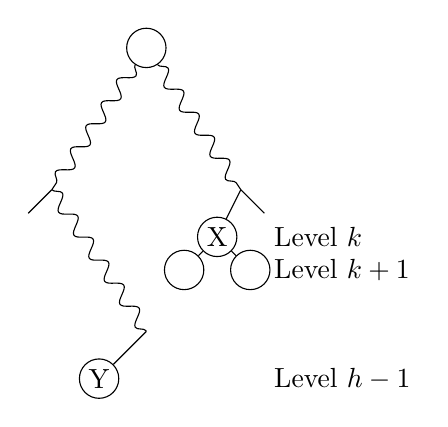
\begin{tikzpicture}[scale=0.6,place/.style={circle,draw, fill=white,inner sep=0pt,minimum size=5mm}]
            \node (x31)  at (1,5) [place] { };
            \draw [decorate,decoration=snake] (x31) -- (-1,2);
            \draw [decorate,decoration=snake] (x31) -- (3,2);
            \draw [] (-1,2) -- (-1.5,1.5);
            \draw [] (3,2) -- (3.5,1.5);
            \node (x21)  at (2.5,1) [place] {X};
            \draw [] (3,2) -- (x21);
            \draw [decorate,decoration=snake] (-1,2) -- (1,-1);
            \node (y)  at (0,-2) [place] {Y};
            \draw [] (1,-1) -- (y);
            \node (y1)  at (1.8,0.3) [place] { };
            \node (y2)  at (3.2,0.3) [place] { };
            \draw [] (x21) -- (y1);
            \draw [] (x21) -- (y2);
            \node (w1)  at (3.5,1) [right] {Level $k$};
            \node (w2)  at (3.5,-2) [right] {Level $h-1$};
            \node (w2)  at (3.5,0.3) [right] {Level $k+1$};
        \end{tikzpicture}
        \label{Fig:ReducingExternalPathLength_B}
    }
    \caption{约简external path长度}
    \label{Fig:ReducingExternalPathLength}
\end{figure*}

我们需要一个决策树中所有从根到叶子路径的平均长度的底限。回顾定义
\ref{Def:ExternalNodeAnd2_tree},如果二叉树每一个节点的度都是0
或者2,则这课二叉树称为\emph{2-tree}。这种树的叶子称为
\emph{external nodes},我们的决策树就是一颗2-tree,他们所有的叶子
都是输出指令,而所有的internal 节点都是比较指令。

回顾定义\ref{Def:ExternalNodeAnd2_tree},树的external path length
是所有根到external节点(也就是输出指令)的path长度的和;它被表示为
$epl$。如果决策树有$L$个叶子,根到叶子的平均长度是$epl/L$。

我们将找到所有的叶子数为$L$的决策树(2-trees)$epl$的底限,在
某一时刻想$L$是固定值。我们可以讨论有$L$个叶子的树当尽可能的平衡
时有最小的$epl$。假设我们有一个高度为$h$的2-tree,它有一个叶子$K$
的深度是$k$,这里$k$比$h$少2或者更多。参看图
\ref{Fig:ReducingExternalPathLength_A}。
图\ref{Fig:ReducingExternalPathLength_B}展示了一个有同样数目叶子的
2-tree但$epl$比较小。我们选择深度是$h-1$的节点$Y$,这不是一个叶子,
移除它的两个孩子,附加到节点$X$上去。叶子的总数没有变,但$epl$变了。
原来树中的3条paths,总长度是$h+h+k$,但现在不再算了(到$Y$的孩子和
到$X$的paths)。新的paths(到$Y$的和到$X$的孩子的),总长度是
$h-1+2(k+1)$。$epl$的变化是$k+1-h$,这个值是非负的,所以$epl$是
减少的。因此如果2-tree在所有$L$个叶子中具有最小的$epl$,则它的external
path length大约是$L\lg(L)$\footnote{译注:也就是平衡树时的情况}。

引理\ref{Lemma:ExternalNodeCount}使得边界更加精确;它规定了(在我们
的上下文中)任意$L$个叶子的决策树有$epl \geq L\lg(L)$,于是到输出指令
节点的平均path length至少是$\lg(L)$。这马上导出下面的定理。

\begin{theorem}\label{Theorem::LowerBoundOfSort}
通过比较排序n个条目的算法使用的平均比较次数至少是$\lg(n!)$,
约是$n\lg n -1.443n$。
\end{theorem}

与最坏情况直接唯一的区别在于平均情况不需要取整到一个整数——平均值可以
不是整数,但是最坏情况必须是整数。尽管我们从没有分析过归并排序的平均
情况,这个一般性的边界允许我们得出结论,归并排序的平均情况不可能比它
的最坏情况低;主要阶的部分一致,次要阶部分只有约$0.5n$的差距。同样的,
快速排序的平均情况对于任意的增强也只能提高大约30\%,比如小心的选择splitting
元素。

\section{堆排序}\label{Sec:HeapSort}
快速排序重新排列原来数组的元素,但是不能保证对一个个问题进行完全的分解,
因此它有一个最坏的情况。归并排序可以保证问题的分解,对最坏的情况下也接近
最优,但是它不能在原来数组重新排列;它需要相当大的辅助的空间。堆排序重新
排列了数组的元素,它的最坏情况$\Theta(n\log n)$,这是最优的增长率,所以综合了
快速排序和归并排序的优点。它的缺点是有比其他两个大的常数因子。但是新版本
的Heapsort减少了常数因子,使得堆排序可以和快速和归并一起竞争了。我们称
这个新版本叫\emph{Accelerated Heapsort}。因此Accelerated Heapsort也是一种排序
的选择方案。

\subsection{堆}
\begin{figure*}[!t]
    \centering
    \subfloat[一颗2-tree]{
        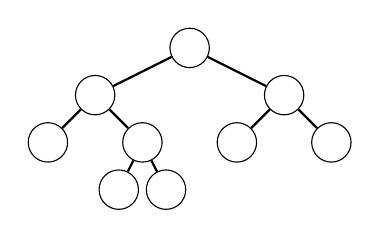
\begin{tikzpicture}[scale=0.6,place/.style={circle,draw, fill=white,inner sep=0pt,minimum size=5mm}]
        \node (x31)  at (4,3) [place] {};
        \node (x21)  at (2,2) [place] {};
        \node (x22)  at (6,2) [place] {};
        \node (x11)  at (1,1) [place] {};
        \node (x12)  at (3,1) [place] {};
        \node (x13)  at (5,1) [place] {};
        \node (x14)  at (7,1) [place] {};
        \node (x03)  at (2.5,0) [place] {};
        \node (x04)  at (3.5,0) [place] {};

        \draw [thick] (x31) -- (x21);
        \draw [thick] (x31) -- (x22);
        \draw [thick] (x21) -- (x11);
        \draw [thick] (x21) -- (x12);
        \draw [thick] (x22) -- (x13);
        \draw [thick] (x22) -- (x14);
        \draw [thick] (x12) -- (x03);
        \draw [thick] (x12) -- (x04);

        \end{tikzpicture}
        \label{Fig:HeapAnd2_tree_A}
    }
    \hfil
    \subfloat[完全二叉树]{
        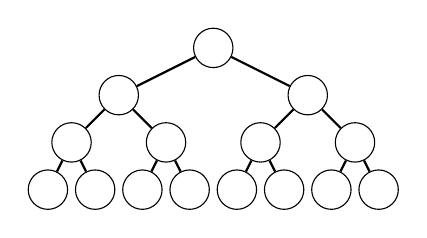
\begin{tikzpicture}[scale=0.6,place/.style={circle,draw, fill=white,inner sep=0pt,minimum size=5mm}]
        \node (x31)  at (4,3) [place] {};
        \node (x21)  at (2,2) [place] {};
        \node (x22)  at (6,2) [place] {};
        \node (x11)  at (1,1) [place] {};
        \node (x12)  at (3,1) [place] {};
        \node (x13)  at (5,1) [place] {};
        \node (x14)  at (7,1) [place] {};
        \node (x01)  at (0.5,0) [place] {};
        \node (x02)  at (1.5,0) [place] {};
        \node (x03)  at (2.5,0) [place] {};
        \node (x04)  at (3.5,0) [place] {};
        \node (x05)  at (4.5,0) [place] {};
        \node (x06)  at (5.5,0) [place] {};
        \node (x07)  at (6.5,0) [place] {};
        \node (x08)  at (7.5,0) [place] {};

        \draw [thick] (x31) -- (x21);
        \draw [thick] (x31) -- (x22);
        \draw [thick] (x21) -- (x11);
        \draw [thick] (x21) -- (x12);
        \draw [thick] (x22) -- (x13);
        \draw [thick] (x22) -- (x14);
        \draw [thick] (x11) -- (x01);
        \draw [thick] (x11) -- (x02);
        \draw [thick] (x12) -- (x03);
        \draw [thick] (x12) -- (x04);
        \draw [thick] (x13) -- (x05);
        \draw [thick] (x13) -- (x06);
        \draw [thick] (x14) -- (x07);
        \draw [thick] (x14) -- (x08);
        \end{tikzpicture}
        \label{Fig:HeapAnd2_tree_B}
    }
    \hfil
    \subfloat[堆1]{
        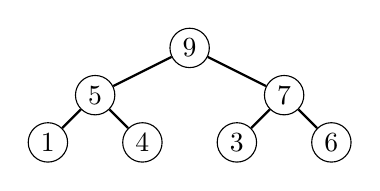
\begin{tikzpicture}[scale=0.6,place/.style={circle,draw, fill=white,inner sep=0pt,minimum size=5mm}]
        \node (x31)  at (4,3) [place] {9};
        \node (x21)  at (2,2) [place] {5};
        \node (x22)  at (6,2) [place] {7};
        \node (x11)  at (1,1) [place] {1};
        \node (x12)  at (3,1) [place] {4};
        \node (x13)  at (5,1) [place] {3};
        \node (x14)  at (7,1) [place] {6};


        \draw [thick] (x31) -- (x21);
        \draw [thick] (x31) -- (x22);
        \draw [thick] (x21) -- (x11);
        \draw [thick] (x21) -- (x12);
        \draw [thick] (x22) -- (x13);
        \draw [thick] (x22) -- (x14);
        \end{tikzpicture}
        \label{Fig:HeapAnd2_tree_C}
    }
    \hfil
    \subfloat[堆2]{
        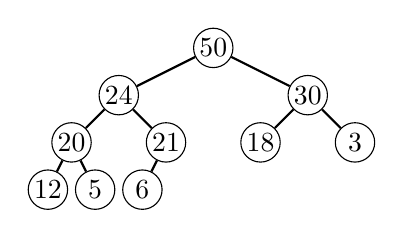
\begin{tikzpicture}[scale=0.6,place/.style={circle,draw, fill=white,inner sep=0pt,minimum size=5mm}]
        \node (x31)  at (4,3) [place] {50};
        \node (x21)  at (2,2) [place] {24};
        \node (x22)  at (6,2) [place] {30};
        \node (x11)  at (1,1) [place] {20};
        \node (x12)  at (3,1) [place] {21};
        \node (x13)  at (5,1) [place] {18};
        \node (x14)  at (7,1) [place] {3};
        \node (x01)  at (0.5,0) [place] {12};
        \node (x02)  at (1.5,0) [place] {5};
        \node (x03)  at (2.5,0) [place] {6};

        \draw [thick] (x31) -- (x21);
        \draw [thick] (x31) -- (x22);
        \draw [thick] (x21) -- (x11);
        \draw [thick] (x21) -- (x12);
        \draw [thick] (x22) -- (x13);
        \draw [thick] (x22) -- (x14);
        \draw [thick] (x11) -- (x01);
        \draw [thick] (x11) -- (x02);
        \draw [thick] (x12) -- (x03);
        \end{tikzpicture}
        \label{Fig:HeapAnd2_tree_D}
    }
    \caption{2-trees,完全二叉树和堆}
    \label{Fig:HeapAnd2_tree}
\end{figure*}

堆排序用到一种叫堆的数据结构,它是一颗特殊的二叉树。堆的定义包括数据结构
和节点上数据的条件,叫做partial order tree property。非正式的,堆结构是
一个完全二叉树,它的叶子节点的右面部分可能不全。
(参见图\ref{Fig:HeapAnd2_tree})堆提供了对ADT优先级队列的的有效
实现(\ref{Sec:ADTPriorityQueue})。在堆中,最高优先级的的数据放在根节点。
根据这种优先排序的观点,根节点可以是最小值(小顶堆)或是最大值(大顶堆)。
对于一个升序的堆排序排序的堆,我们需要建立一个大顶堆,我们将从这方面来
描述堆,其他情况我们可能需要建立一个小顶堆。

我们将使用两个术语,S是一个关键字是线型的元素的集合,T是高度为h的二叉树,
它的节点属于S。

\begin{definition}
堆结构

二叉树T是一个\emph{堆结构},当且仅当它符合下面的条件:
\begin{enumerate}
\item T的高度至少为h-1且为完全二叉树
\item 所有的叶子的深度为h或h-1
\item 所有到深度为h的叶子的路径都在到深度为h-1的叶子的路径的左侧
\end{enumerate}

深度为h-1的最右边的内部节点可能有左孩子,没有右孩子。其他的内部节点
都有2个孩子。堆结构的另一个名字是\emph{左完全}二叉树。
\end{definition}

\begin{definition}
partial order tree property

树T是(大的)partial order tree 当且仅当每一个节点都大于等于它的每一个
孩子(如果存在孩子)。
\end{definition}

一颗完全二叉树是一个堆结构。当添加新元素到堆时,他们必须从左自右加到
最底层,而且如果移除节点,必须一处最底层最右边的节点,如果移除节点之后
仍然是一个堆的话。注意根必须是堆中最大的元素。

\subsection{堆排序的策略}
如果要排序的元素在一个堆中,则我们通过重复下面的过程构造一个逆序列:
把堆的根元素(剩下的最大的元素)移出,移走了最大元素之后重新排列元素
使得剩下的元素仍然是一个堆。这个操作就是优先级队列ADT的deleteMax操作。
(我们可以用小顶堆来得到一个升序序列,之所以用大顶堆是因为我们在
\ref{Sec:ImplementationOfHeapAndHeapsort}要学习一种更有效率的实现方法。)

既然第一步是要建立一个堆,之后不断调用deleteMax(这个函数调用某个重新
构造一个逆序列堆排列元素),这看起来不象一个得到排序算法的有效的策略。
但是把它发展成一个排序算法很容易。因此我们在这里大概的给出策略,等会
给出细节。和往常一样,我们假设n个元素存放在数组E中,但是这次我们假设
索引从$1, \cdots,n$,因为这样我们看堆的实现方式时比较清楚。暂时我们假设
堆(叫H)在别处。

\begin{figure*}[!t]
    \centering
    \subfloat[堆]{
        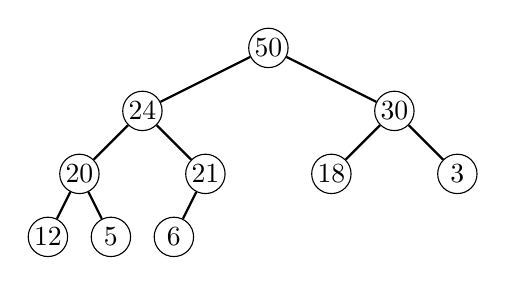
\begin{tikzpicture}[scale=0.8,place/.style={circle,draw, fill=white,inner sep=0pt,minimum size=5mm}]
        \node (x31)  at (4,3) [place] {50};
        \node (x21)  at (2,2) [place] {24};
        \node (x22)  at (6,2) [place] {30};
        \node (x11)  at (1,1) [place] {20};
        \node (x12)  at (3,1) [place] {21};
        \node (x13)  at (5,1) [place] {18};
        \node (x14)  at (7,1) [place] {3};
        \node (x01)  at (0.5,0) [place] {12};
        \node (x02)  at (1.5,0) [place] {5};
        \node (x03)  at (2.5,0) [place] {6};
        \draw [thick] (x31) -- (x21);
        \draw [thick] (x31) -- (x22);
        \draw [thick] (x21) -- (x11);
        \draw [thick] (x21) -- (x12);
        \draw [thick] (x22) -- (x13);
        \draw [thick] (x22) -- (x14);
        \draw [thick] (x11) -- (x01);
        \draw [thick] (x11) -- (x02);
        \draw [thick] (x12) -- (x03);
        \end{tikzpicture}
        \label{Fig:ReestablishingHeap_A}
    }
    \hfil
    \subfloat[根的元素已经被移除;底层最右边叶子被移除了。$K=6$需要再次插入堆。]{
        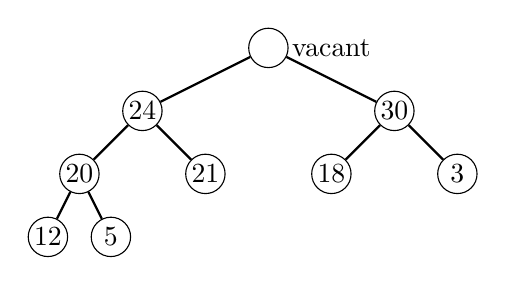
\begin{tikzpicture}[scale=0.8,place/.style={circle,draw, fill=white,inner sep=0pt,minimum size=5mm}]
        \node (x31)  at (4,3) [place] { };
        \node (x21)  at (2,2) [place] {24};
        \node (x22)  at (6,2) [place] {30};
        \node (x11)  at (1,1) [place] {20};
        \node (x12)  at (3,1) [place] {21};
        \node (x13)  at (5,1) [place] {18};
        \node (x14)  at (7,1) [place] {3};
        \node (x01)  at (0.5,0) [place] {12};
        \node (x02)  at (1.5,0) [place] {5};

        \draw [thick] (x31) -- (x21);
        \draw [thick] (x31) -- (x22);
        \draw [thick] (x21) -- (x11);
        \draw [thick] (x21) -- (x12);
        \draw [thick] (x22) -- (x13);
        \draw [thick] (x22) -- (x14);
        \draw [thick] (x11) -- (x01);
        \draw [thick] (x11) -- (x02);
        \draw (5,3) node {vacant};
        \end{tikzpicture}
        \label{Fig:ReestablishingHeap_B}
    }
    \hfil
    \subfloat[vacant较大的孩子,30,比$K$大,所以30上移,vacant下移。]{
        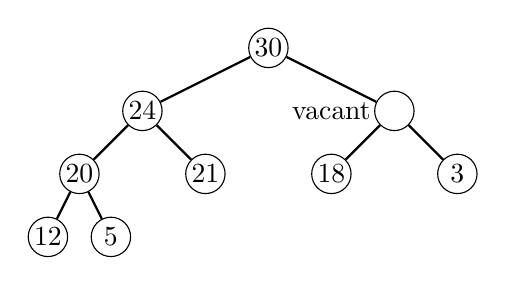
\begin{tikzpicture}[scale=0.8,place/.style={circle,draw, fill=white,inner sep=0pt,minimum size=5mm}]
        \node (x31)  at (4,3) [place] {30};
        \node (x21)  at (2,2) [place] {24};
        \node (x22)  at (6,2) [place] { };
        \node (x11)  at (1,1) [place] {20};
        \node (x12)  at (3,1) [place] {21};
        \node (x13)  at (5,1) [place] {18};
        \node (x14)  at (7,1) [place] {3};
        \node (x01)  at (0.5,0) [place] {12};
        \node (x02)  at (1.5,0) [place] {5};
        \draw [thick] (x31) -- (x21);
        \draw [thick] (x31) -- (x22);
        \draw [thick] (x21) -- (x11);
        \draw [thick] (x21) -- (x12);
        \draw [thick] (x22) -- (x13);
        \draw [thick] (x22) -- (x14);
        \draw [thick] (x11) -- (x01);
        \draw [thick] (x11) -- (x02);
        \draw (5,2) node {vacant};
        \end{tikzpicture}
        \label{Fig:ReestablishingHeap_C}
    }
    \hfil
    \subfloat[vacant较大的孩子,18,比$K$大,所以18上移,vacant下移。]{
        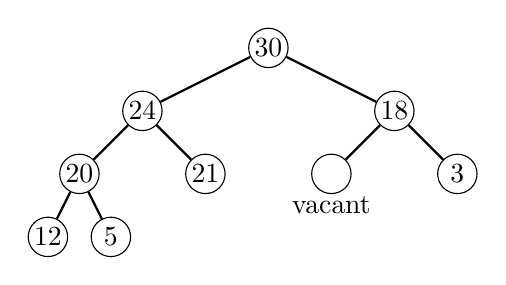
\begin{tikzpicture}[scale=0.8,place/.style={circle,draw, fill=white,inner sep=0pt,minimum size=5mm}]
        \node (x31)  at (4,3) [place] {30};
        \node (x21)  at (2,2) [place] {24};
        \node (x22)  at (6,2) [place] {18};
        \node (x11)  at (1,1) [place] {20};
        \node (x12)  at (3,1) [place] {21};
        \node (x13)  at (5,1) [place] { };
        \node (x14)  at (7,1) [place] {3};
        \node (x01)  at (0.5,0) [place] {12};
        \node (x02)  at (1.5,0) [place] {5};
        \draw [thick] (x31) -- (x21);
        \draw [thick] (x31) -- (x22);
        \draw [thick] (x21) -- (x11);
        \draw [thick] (x21) -- (x12);
        \draw [thick] (x22) -- (x13);
        \draw [thick] (x22) -- (x14);
        \draw [thick] (x11) -- (x01);
        \draw [thick] (x11) -- (x02);
        \draw (5,0.5) node {vacant};
        \end{tikzpicture}
        \label{Fig:ReestablishingHeap_D}
    }
    \hfil
    \subfloat[最后,既然vacant已经是叶子了,$K$插入。]{
        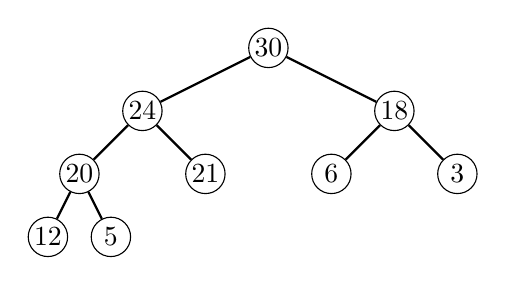
\begin{tikzpicture}[scale=0.8,place/.style={circle,draw, fill=white,inner sep=0pt,minimum size=5mm}]
        \node (x31)  at (4,3) [place] {30};
        \node (x21)  at (2,2) [place] {24};
        \node (x22)  at (6,2) [place] {18};
        \node (x11)  at (1,1) [place] {20};
        \node (x12)  at (3,1) [place] {21};
        \node (x13)  at (5,1) [place] {6};
        \node (x14)  at (7,1) [place] {3};
        \node (x01)  at (0.5,0) [place] {12};
        \node (x02)  at (1.5,0) [place] {5};
        \draw [thick] (x31) -- (x21);
        \draw [thick] (x31) -- (x22);
        \draw [thick] (x21) -- (x11);
        \draw [thick] (x21) -- (x12);
        \draw [thick] (x22) -- (x13);
        \draw [thick] (x22) -- (x14);
        \draw [thick] (x11) -- (x01);
        \draw [thick] (x11) -- (x02);
        \end{tikzpicture}
        \label{Fig:ReestablishingHeap_E}
    }
    \caption{删除根的元素,并重建partial order tree属性}
    \label{Fig:ReestablishingHeap}
\end{figure*}

\begin{lstlisting}[language={Java}, keywordstyle=\color{blue!70}, commentstyle=\color{red!50!green!50!blue!50}]
heapSort(E, n)
    Construct H from E, E`是要排序的n个元素的集合;`
    for(i=0;i>=1; i--)
        curMax=getMax(H);
        deleteMax(H);
        E[i]=curMax;
\end{lstlisting}

图\ref{Fig:ReestablishingHeap}的第一和最后的图片展示了一个例子,
分别是for循环开始和结束之后的情况。中间的图片展示了deleteMax和
fixHeap调用时重新排列的步骤,fixHeap由deleteMax调用。
\begin{lstlisting}[language={Java}, keywordstyle=\color{blue!70}, commentstyle=\color{red!50!green!50!blue!50}]
deleteMax(H)
    `拷贝H最底层最右边的元素到K。`
    `删除H最底层最右边的元素。`
    fixHeap(H,K);
\end{lstlisting}
显然,几乎所有的工作都由fixHeap完成。

我们现在需要一个算法来构造堆,还需要一个算法来fixHeap。因为fixHeap
可以用来解决构造堆的问题,所以我们下面考虑fixHeap。

\subsection{修正堆}\label{Sec:FixHeap}
fixHeap过程恢复堆结构的partial order tree property,堆结构必须是除了
根以外其余部分都是符合要求的。特定的,当fixHeap开始的时候,我们有一个
根是“空位”的堆结构。两个子树都是partial order tree,而我们有一个额外
的元素,叫K,要插入到堆中。既然根是一个空位,我们从根开始,令
K(空位节点)下降到它正确的位置。到空位正确的位置之后,
K(准确的说是K的关键字)必须大于或等于它的两个孩子,这样每一步中K
需要和当前空位节点的大的孩子比较。如果K大于(或是等于)它就要可以
被插入到等前空位节点处。否则,大的孩子被移动到空位,重复之。

\begin{example}
FixHeap实战

fixHeap的动作展示在图4.18的第二到第五图片中。稍微回退一点,
第一图片展示了初始时的状态,即4.8.2小节中heapSort的for循环开始时
的状态。首先,fixHeap将H的根关键字50拷贝到curMax,使得树的根是
一个空位;然后,它调用deleteMax,它将最底层最右边的关键字6拷贝到K,
实际的删除该节点。

这就到了第二图片,这是fixHeap(H,K)开始。空位节点的大的孩子是节点30,
这比K大,所以30移到空位位置,空位下降,到第三图片。同样的,空位
节点的大的孩子仍然大于K,所以空位节点继续下降。下一次,空位节点是
一个叶子,所以K可以被插入到这个位置,H的partial order tree property
就恢复了。
\end{example}

尽管堆的树结构是其本质且容易理解HeapSort,我们之后将用数组来
表示堆和子堆,而没有显式的边。

\begin{algorithm}
FixHeap (Outline)

\noindent{\textbf{\emph{输入:}}}一个非空二叉树带有一个“空位”根,且它
的左子树和右子树都是partial order树,待插入元素K。H的type叫堆。
H的节点假设类型为Element。

\noindent{\textbf{\emph{输出:}}}一个二叉树H,其元素是K和原来H的元素,
满足partial order tree property。

\noindent{\textbf{\emph{注意:}}}H的结构不改变,但是节点的内容改变。
\end{algorithm}
\begin{lstlisting}[language={Java}, keywordstyle=\color{blue!70}, commentstyle=\color{red!50!green!50!blue!50}]
fixHeap(H, K)  //OUTLINEA
{
    if(`H是叶子`)
        `插入K到H的根上`
    else
        `设置largerSubHeap 成leftSubtree(H)或rightSubtree(H),
        选择两者中根的关键字大的。只要rightSubtree不是空,则会有一次关键字比较。`
        if( K.key >= root(largerSubHeap).key)
            `将K插入H的根`
        else
        {
            `插入root(largerSubHeap) 到H的根`;
            fixHeap(largerSubHeap, K);
        }
        return;
}
\end{lstlisting}

\begin{lemma}
fixHeap过程对于高度是h的堆在最坏情况下比较关键字2h次。

{\textbf{\emph{证明}}} 每一次过程调用最多有两次关键字
比较,每次递归调用树高减少1.(在决定largerSubHeap时有
一次隐式比较。)
\end{lemma}

\subsection{构造堆}
假设我们开始把所有的元素都任意的放入堆;就是说,
partial order tree property对于任意子树都不是必须的。fixHeap算法可以
通过分而治之策略来建立partial order tree property。两个子树可以被
递归转换成堆,然后调用fixHeap来将根元素下降到它正确的位置,因此合并
两个子堆和根就成了一个堆。基本情况是由一个节点组成的树(例如一个叶子);
它已经是一个堆了。下面的算法就是这种思想。

\begin{algorithm}
构造堆

\noindent{\textbf{\emph{输入:}}}堆结构H但是不一定符合partial order tree property。

\noindent{\textbf{\emph{输出:}}}有相同元素的H,已经重新排列使之满足partial order tree property。
\end{algorithm}
%\begin{lstlisting}[language={Java}, keywordstyle=\color{blue!70}, commentstyle=\color{red!50!green!50!blue!50}]
%void constructHeap(H)
%{
%    if (`H 不是叶子`)
%    {
%        constructHeap(`H的左子树`);
%        constructHeap(`H的右子树`);
%        `Element K=H的根`;
%        fixHeap(H, K);
%    }
%    return;
%}
%\end{lstlisting}
如果我们拆开这个分而治之的算法,我们会看到实际的工作从靠近叶子的
节点开始。(这是一种后序遍历。)参见图4.19。练习4.38要求你实现
一个迭代版本的constructHeap。

\subsubsection{正确性}
定理 4.13 过程constructHeap为它的参数H建立partial order tree property。

\subsubsection{最坏情况分析}
constructHeap的递归等式依赖于fixHeap耗费的时间。定义问题的规模
是n,n是堆结构H中节点的数量,我们看到fixHeap需要大约2lg(n)次关键字
比较。令r表示H右子堆的节点的数目。我们有
\begin{displaymath}
W(n)=W(n-r-1)+W(r)+2\lg(n)  \mbox{对于} n>1
\end{displaymath}
尽管堆是尽可能平衡的,r可以小到n/3。因此,当costructHeap是分而治之
算法时,它的两个子问题不一定是相等的。对于任意的n在数学上解决这个
递归式子有点困难。我们先解决$N=2^d-1$时的,就是说是一颗完全二叉树,
则对于n在N/2到N之间,W(N)是W(n)的上界。

对于N=2d-1,左子树和右子树的节点数量是相等的,所以递归等式变为
\begin{displaymath}
W(N)=2W(\frac{1}{2}(N-1))+2\lg(N)  \mbox{对于} N>1
\end{displaymath}
现在使用Master定理(定理3.17)。我们令b=2,c=2(N/2与(N-1)/2之间的
区别可以忽略),E=1,以及f(N)=2lg(N)。现在选$\varepsilon=0.1$(或者
任何小于1的小数)适用定理的情况1:$2\lg(N)\in O(n^{0.9})$。
则$W(N)=\Theta(N)$。

现在,回到一般的n,既然$N\leq 2n$,$W(n)\leq W(N)\in \Theta(2n)=\Theta(n)$。
因此,构造堆是线型时间!(另一个方法在练习4.39中。)

现在仍然不清楚Heapsort是一个好的算法;它似乎需要额外的空间。下面
考虑堆的实现。

\subsection{堆的实现和堆排序}\label{Sec:ImplementationOfHeapAndHeapsort}
二叉树通常用链式结构实现,每个节点包含指针(或是其他种类的引用)指向
它的子树。设置和使用每个结构需要额外的时间和额外的空间存放指针。但是,
我们可以完全不用指针来存储和使用堆。在堆中,只有d-1层是满的情况下d层
才可能有节点,所以一个堆可以可以按层存放在数组中,每一层从左自右一次
存放节点。图4.20显示了如何存放图4.17中的两个堆。用这个方案,我们必须
能快速的找到一个节点的子节点,以及快速的决定一个节点是不是叶子。将根
存放在索引1,而不是0,是很重要的,这关系到我们将要讲到的公式。

\subsubsection{堆排序分析}
\subsection{加速堆排序}
回忆一下,fixHeap处理根是空位,但是根的两个子树都满足partial order
tree property。一个新的节点将插入,但是它可能太小不能放在根的位置。
这个元素下降到左或右子树,直到它合适的位置。

假设一个关键字开始的时候位置太低,就是说,对于它当前的位置它大了。
bubbleUpHeap将它向根"升起"。事实上,"升起"会更简单,因为,元素只需要
与它的父节点比较--不需要决定左孩子大还是右孩子大。bubbleUpHeap过程是
对fixHeap(算法4.9)的自然的补充。在写出bubbleUpHeap的细节之后,我们
将看到如何使用扩展因子来将Heapsort加速大约一倍。

我们继续假设是大顶堆,因为这是Heapsort使用的类型。准确的说,bubbleUpHeap
将给出元素K和一个空位位置,这样将元素放到空位的位置可能太低;
K可能大于它的父节点。

过程让空位到根的路径上的小的元素下降,空位上升,知道为新元素找到
正确的位置。(对于索引i,父节点是$\lfloor i/2 \rfloor$ 。)操作类似
于插入排序中将一个新元素插入到前面已经有序序列中的过程。

\begin{algorithm}
Bubble-Up Heap

输入:一个表示堆结构的数组;整数表示的root和vacant,一个元素K要插入
到vacant或是vacant的祖先,并且保持E的partial order tree property。作为一
个precondition,如果不算vacant,E有partial order tree property。

输出:以root为根且K已经插入的子堆,且有partial order tree property。

注意:E的结构没有改变,但是它的节点的内容改变了。

\end{algorithm}

\begin{lstlisting}[language={Java}, keywordstyle=\color{blue!70}, commentstyle=\color{red!50!green!50!blue!50}]
void bubbleUpHeap(Element[] E, int root, Element K, int vacant)
{
    if(vacant==root)
        E[vacant]=K;
    else
    {
        int parent= vacant/2;
        if(K.key<=E[parent].key)
            E[vacant]=k;
        else
        {
            E[vacant]=E[parent];
            bubbleUpHeap(E, root, K, parent);
        }
    }
}
\end{lstlisting}

将一个元素通过bubbleUpHeap升起一层只需要一次比较。算法4.10可以用
来实现在堆中插入一个元素(参见练习4.41)。

联合bubbleUpHeap对fixHeap做一个简单的修改,允许我们将Heapsort比较
的次数减约一半左右。这使得Heapsort可以在比较次数上和归并排序竞争了,
他们的最坏情况下的系数一样了(1)。元素的移动次数,没有减少,但是
数量级和归并一样了。堆排序的优点是不用辅助数组。

主要的思想是简单的。fixHeap将一个元素下降一层需要两次比较。但是我们
可以避免其中一次比较--

\subsubsection{分析}
本质上,

\section{四种排序算法的比较}
\begin{table}
\centering
\begin{tabular}{lccl}
    \hline
    算法   &最坏情况 &平均情况 &空间使用 \\
    \hline
    插入排序   &$n^2/2$    &$\Theta(n^2)$     &in place\\
    快速排序   &$n^2/2$    &$\Theta(n\log n)$ &额外空间和$\log n$成比例\\
    归并排序   &$n\lg n$   &$\Theta(n\log n)$ &额外空间和$n$成比例\\
    堆排序     &$2n\lg n$  &$\Theta(n\log n)$ &in place\\
    加速堆排序 &$n\lg n$   &$\Theta(n\log n)$ &in place\\
    \hline
\end{tabular}
\caption{四种排序算法分析的结果。Entries are number of comparisons and include the leading terms only。}
\label{Table:CompareOf4Algorithm} \centering
\end{table}
表\ref{Table:CompareOf4Algorithm}综合了迄今为止讨论过的四种排序算法分析的结果。
尽管归并排序在最坏情况下最接近最优,但是有比较次数更少的算法。
\ref{Sec:LowerBoundsForSortingByComparisonOfKeys}节得到的底限是相当好的。它对于
有些n的值是很精确的;就是说,排序$\lceil\lg n!\rceil$次比较就足够,对于一些n的值。
也知道$\lceil\lg n!\rceil$并不是对于所有n的值都足够。例如$\lceil\lg 12!\rceil=29$,
但是已经证明排序12个元素在最坏情况下至少需要30次比较。参看本章后面的Notes和
References,哪种排序算法在最坏情况下最接近底限。

\section{Shell排序}\label{Sec:ShellSort}
Shell排序(以发明者Donald Shell 命名)用的技术是有趣的,而且算法易于编程,
运行的相当快。只是它的分析是非常困难,而且是不完全的。
\subsection{算法}
Shell排序
\subsection{分析和注意事项}

\section{基数排序}\label{Sec:RadixSorting}
对于\ref{Sec:InsertSort}到\ref{Sec:ShellSort}的排序算法,对于关键字的假设
只有一个:他们是线型的集合。基本的操作是比较两个关键字。如果我们对关键字
作更多的假设,我们能可以对关键字做其他的操作。本节学习一种新的算法,叫
“桶排序”,“基数排序”或是“分配排序”
\subsection{使用关键字的属性}
假设关键字是打印在卡片上的名字,一个卡片一个名字。为了用手将他们按字母
顺序排序,我们首先根据首字母将他们分成26堆,或者按几个字母一堆分好;用
其他方法将每一堆卡片按字母顺序排好,比如类似插入排序;最后合并排好序的堆。
如果关键字是5位十进制树,我们可以根据第一位将他们分成10堆。如果关键字是
1到m之间的整数,我们可以每间隔k分一堆,[1, m/k],[m/k+1, 2m/k]等等。上面
的例子中,都是根据检查关键字的一个单独字母或一位数字,或是与预先定好的
值比较,来将关键字分发到不同的堆中。然后再将堆单独排序在组合。以这种
方式排序的算法与前面讨论所的算法都不同,因为要使用这种方法我们必须知道
关键字的结构或是顺序。

我们将在后面展示\emph{基数排序算法}的细节。为了区分同类新的其他算法,我们使用
“桶排序”做这类算法的通用名字。

\subsubsection{桶排序有多块}
一个桶排序算法有3步:
\begin{enumerate}
\item 分发关键字
\item 单独排序桶
\item 合并桶
\end{enumerate}
每一步工作的类型都是不同的,所以我们选一个通用的基本操作来计数的策略
不好用了。假设有k个桶。

在分发阶段,算法检查每个关键字一次(不管是检查某个特定的位域,或是将关键字
与常数个特定值比较。)然后算法决定关键字属于那个桶。这一步可能牵涉到拷贝
关键字或是设置指针引用什么的。第一步的一个合理的实现应该将操作步数控制在$\Theta(n)$。

为了排序桶,假设我们使用一种基于比较关键字的排序算法,即对于m个元素的桶需
要$S(m)$次比较。令$n_i$是第i个桶中的元素个数。第二步算法要做$\Sigma_{i=1}^kS(n_i)$
次比较。

第三步,合并桶,最坏情况下需要将所有的元素从桶拷贝到一个list中;操作的数量是$O(n)$。

因此主要的工作是在排序桶时。假设S(m)在Θ(mlogm)。则如果关键字均匀的
分布在桶中,算法在第二步要做ck(n/k)lg(n/k)=cnlg(n/k)次比较,这里c是一个
依赖于在桶中使用排序算法的常数。增加桶的数量k将减少比较的数量。如果我们
选k=n/10,则要做nlg10次比较,桶排序的时间将在n的线性之内,假设关键字是均匀的
分发且第一步的运行时间不依赖于k的话。(As a caveat, the fewer elements pre bucket,
the less likely it is that the distribution will be even。)但是在最坏的情况下,
所有的元素都装进一个桶里面,第二步中要对整个list排序,而第一步和第三步都变成了浪费。
因此在最坏情况下,桶排序会变的极度低效。如果关键字的分布是可以预先知道的,则可以
调整每个桶保存关键字的范围,使得所有的桶都接受近似相等数量的元素。

桶排序需要的空间依赖于桶是如何存储的。如果每一个桶都是连续空间的集合(例如数组),
则每一个桶都必须分配足够的空间以存储一个桶的最多可能的元素数量,也就是所有的元素n。
因此排序n个元素可能需要$kn$个空间。随着桶数量的增加,算法的速度增加但是使用的空间也
随之增加。链表可能会好点;仅需要$\Theta(k+n)$的空间(n个元素占用n个空间,k个表头
占用k个空间)。将关键字分发到桶中可能需要构造list的节点。但是每个桶中的元素如何排序
呢?快速排序和归并排序,先前讨论的两种最快的排序方法,都可以在链表上简单的实现(参看
练习4.22和连续4.28)。如果桶的数量很大,桶内的元素的数量很少,可以使用慢一点的算法。
插入排序也也可以简单的修改之后就用于链表(参看练习4.11)。如果每个桶都是大约n/k个元素,
归并排序对每个桶平均做大约$(n/k)(\lg(n)-\lg(k))$次比较,总共做$n(\lg(n)-\lg(k))$次比较。
再次强调,随着k增加,速度也增加,但是空间也增加。

你可能奇怪为什么我们不使用桶排序算法递归的创建更小的桶。这里有几个原因。簿记工作马上
就会超出控制;指向桶头的指针以及最后合并元素需要信息不得不不断的进栈出栈。由于每一个
递归调用都要簿记信息,算法不能依赖于最后将问题分解成一个桶装一个元素,所以将用到其他
的排序算法来排序小的桶。因此如果一开始就使用了合适多的桶,在递归桶排序就会得到的少,
失去的多。但是尽管递归分发关键字到桶是低效的,但有时利用这种思想还是很有用的。

\subsection{基数排序}
\begin{figure*}[!t]
    \centering
    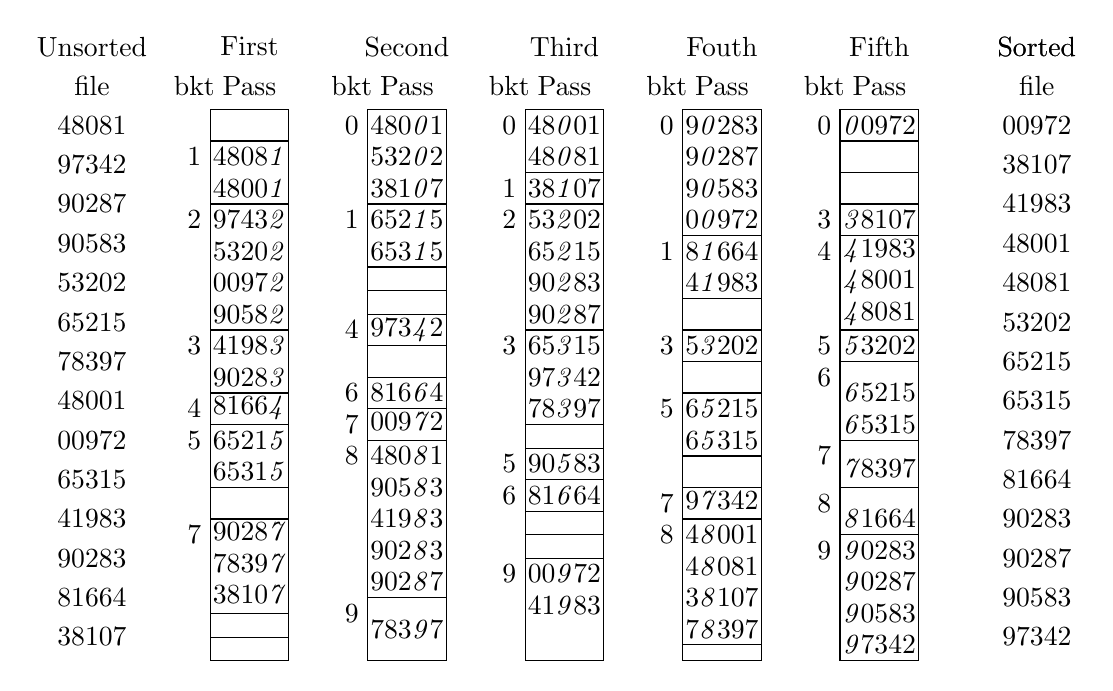
\begin{tikzpicture}[scale=1,place/.style={minimum height=2ex}]
        \node at (0,0) [place] {Unsorted};
        \node at (0,-0.5) [place] {file};
        \node at (0,-1) [place] {48081};
        \node at (0,-1.5) [place] {97342};
        \node at (0,-2) [place] {90287};
        \node at (0,-2.5) [place] {90583};
        \node at (0,-3) [place] {53202};
        \node at (0,-3.5) [place] {65215};
        \node at (0,-4) [place] {78397};
        \node at (0,-4.5) [place] {48001};
        \node at (0,-5) [place] {00972};
        \node at (0,-5.5) [place] {65315};
        \node at (0,-6) [place] {41983};
        \node at (0,-6.5) [place] {90283};
        \node at (0,-7) [place] {81664};
        \node at (0,-7.5) [place] {38107};

        \foreach \x/\c in{2/First, 4/Second, 6/Third, 8/Fouth, 10/Fifth}
            \node at (\x,0) [place] {\c};
        \foreach \x/\c in{2/Pass, 4/Pass, 6/Pass, 8/Pass, 10/Pass}
            \node at (\x,-0.5) [place] {\c};
        \foreach \x/\c in{1.3/bkt, 3.3/bkt, 5.3/bkt, 7.3/bkt, 9.3/bkt}
            \node at (\x,-0.5) [place] {\c};
        \foreach \x in{1.5, 3.5, 5.5, 7.5, 9.5}
            \draw (\x,-0.8) rectangle (\x+1,-7.8);

        % First
        \draw (1.5,-1.2) -- (1.5+1, -1.2);
        \node at (1.3,-1.4) [place] {1};
        \node at (2,-1.4) [place] {4808\emph{1}};
        \node at (2,-1.8) [place] {4800\emph{1}};
        \draw (1.5,-2.0) -- (1.5+1, -2.0);
        \node at (1.3,-2.2) [place] {2};
        \node at (2,-2.2) [place] {9743\emph{2}};
        \node at (2,-2.6) [place] {5320\emph{2}};
        \node at (2,-3.0) [place] {0097\emph{2}};
        \node at (2,-3.4) [place] {9058\emph{2}};
        \draw (1.5,-3.6) -- (1.5+1, -3.6);
        \node at (1.3,-3.8) [place] {3};
        \node at (2,-3.8) [place] {4198\emph{3}};
        \node at (2,-4.2) [place] {9028\emph{3}};
        \draw (1.5,-4.4) -- (1.5+1, -4.4);
        \node at (1.3,-4.6) [place] {4};
        \node at (2,-4.6) [place] {8166\emph{4}};
        \draw (1.5,-4.8) -- (1.5+1, -4.8);
        \node at (1.3,-5.0) [place] {5};
        \node at (2,-5.0) [place] {6521\emph{5}};
        \node at (2,-5.4) [place] {6531\emph{5}};
        \draw (1.5,-5.6) -- (1.5+1, -5.6);
        \draw (1.5,-6.0) -- (1.5+1, -6.0);
        \node at (1.3,-6.2) [place] {7};
        \node at (2,-6.2) [place] {9028\emph{7}};
        \node at (2,-6.6) [place] {7839\emph{7}};
        \node at (2,-7.0) [place] {3810\emph{7}};
        \draw (1.5,-7.2) -- (1.5+1, -7.2);
        \draw (1.5,-7.5) -- (1.5+1, -7.5);

        % Second
        \node at (3.3,-1) [place] {0};
        \node at (4,-1) [place] {480\emph{0}1};
        \node at (4,-1.4) [place] {532\emph{0}2};
        \node at (4,-1.8) [place] {381\emph{0}7};
        \draw (3.5,-2.0) -- (3.5+1, -2.0);
        \node at (3.3,-2.2) [place] {1};
        \node at (4,-2.2) [place] {652\emph{1}5};
        \node at (4,-2.6) [place] {653\emph{1}5};
        \draw (3.5,-2.8) -- (3.5+1, -2.8);
        \draw (3.5,-3.1) -- (3.5+1, -3.1);
        \draw (3.5,-3.4) -- (3.5+1, -3.4);
        \node at (3.3,-3.6) [place] {4};
        \node at (4,-3.6) [place] {973\emph{4}2};
        \draw (3.5,-3.8) -- (3.5+1, -3.8);
        \draw (3.5,-4.2) -- (3.5+1, -4.2);
        \node at (3.3,-4.4) [place] {6};
        \node at (4,-4.4) [place] {816\emph{6}4};
        \draw (3.5,-4.6) -- (3.5+1, -4.6);
        \node at (3.3,-4.8) [place] {7};
        \node at (4,-4.8) [place] {009\emph{7}2};
        \draw (3.5,-5.0) -- (3.5+1, -5.0);
        \node at (3.3,-5.2) [place] {8};
        \node at (4,-5.2) [place] {480\emph{8}1};
        \node at (4,-5.6) [place] {905\emph{8}3};
        \node at (4,-6.0) [place] {419\emph{8}3};
        \node at (4,-6.4) [place] {902\emph{8}3};
        \node at (4,-6.8) [place] {902\emph{8}7};
        \draw (3.5,-7.0) -- (3.5+1, -7.0);
        \node at (3.3,-7.2) [place] {9};
        \node at (4,-7.4) [place] {783\emph{9}7};

        % Third
        \node at (5.3,-1) [place] {0};
        \node at (6,-1) [place] {48\emph{0}01};
        \node at (6,-1.4) [place] {48\emph{0}81};
        \draw (5.5,-1.6) -- (5.5+1, -1.6);
        \node at (5.3,-1.8) [place] {1};
        \node at (6,-1.8) [place] {38\emph{1}07};
        \draw (5.5,-2.0) -- (5.5+1, -2.0);
        \node at (5.3,-2.2) [place] {2};
        \node at (6,-2.2) [place] {53\emph{2}02};
        \node at (6,-2.6) [place] {65\emph{2}15};
        \node at (6,-3.0) [place] {90\emph{2}83};
        \node at (6,-3.4) [place] {90\emph{2}87};
        \draw (5.5,-3.6) -- (5.5+1, -3.6);
        \node at (5.3,-3.8) [place] {3};
        \node at (6,-3.8) [place] {65\emph{3}15};
        \node at (6,-4.2) [place] {97\emph{3}42};
        \node at (6,-4.6) [place] {78\emph{3}97};
        \draw (5.5,-4.8) -- (5.5+1, -4.8);
        \draw (5.5,-5.1) -- (5.5+1, -5.1);
        \node at (5.3,-5.3) [place] {5};
        \node at (6,-5.3) [place] {90\emph{5}83};
        \draw (5.5,-5.5) -- (5.5+1, -5.5);
        \node at (5.3,-5.7) [place] {6};
        \node at (6,-5.7) [place] {81\emph{6}64};
        \draw (5.5,-5.9) -- (5.5+1, -5.9);
        \draw (5.5,-6.2) -- (5.5+1, -6.2);
        \draw (5.5,-6.5) -- (5.5+1, -6.5);
        \node at (5.3,-6.7) [place] {9};
        \node at (6,-6.7) [place] {00\emph{9}72};
        \node at (6,-7.1) [place] {41\emph{9}83};

        %Fourth
        \node at (7.3,-1) [place] {0};
        \node at (8,-1) [place] {9\emph{0}283};
        \node at (8,-1.4) [place] {9\emph{0}287};
        \node at (8,-1.8) [place] {9\emph{0}583};
        \node at (8,-2.2) [place] {0\emph{0}972};
        \draw (7.5,-2.4) -- (7.5+1, -2.4);
        \node at (7.3,-2.6) [place] {1};
        \node at (8,-2.6) [place] {8\emph{1}664};
        \node at (8,-3.0) [place] {4\emph{1}983};
        \draw (7.5,-3.2) -- (7.5+1, -3.2);
        \draw (7.5,-3.6) -- (7.5+1, -3.6);
        \node at (7.3,-3.8) [place] {3};
        \node at (8,-3.8) [place] {5\emph{3}202};
        \draw (7.5,-4.0) -- (7.5+1, -4.0);
        \draw (7.5,-4.4) -- (7.5+1, -4.4);
        \node at (7.3,-4.6) [place] {5};
        \node at (8,-4.6) [place] {6\emph{5}215};
        \node at (8,-5.0) [place] {6\emph{5}315};
        \draw (7.5,-5.2) -- (7.5+1, -5.2);
        \draw (7.5,-5.6) -- (7.5+1, -5.6);
        \node at (7.3,-5.8) [place] {7};
        \node at (8,-5.8) [place] {9\emph{7}342};
        \draw (7.5,-6.0) -- (7.5+1, -6.0);
        \node at (7.3,-6.2) [place] {8};
        \node at (8,-6.2) [place] {4\emph{8}001};
        \node at (8,-6.6) [place] {4\emph{8}081};
        \node at (8,-7.0) [place] {3\emph{8}107};
        \node at (8,-7.4) [place] {7\emph{8}397};
        \draw (7.5,-7.6) -- (7.5+1, -7.6);

        %Fifth
        \node at (9.3,-1) [place] {0};
        \node at (10,-1) [place] {\emph{0}0972};
        \draw (9.5,-1.2) -- (9.5+1, -1.2);
        \draw (9.5,-1.6) -- (9.5+1, -1.6);
        \draw (9.5,-2.0) -- (9.5+1, -2.0);
        \node at (9.3,-2.2) [place] {3};
        \node at (10,-2.2) [place] {\emph{3}8107};
        \draw (9.5,-2.4) -- (9.5+1, -2.4);
        \node at (9.3,-2.6) [place] {4};
        \node at (10,-2.6) [place] {\emph{4}1983};
        \node at (10,-3.0) [place] {\emph{4}8001};
        \node at (10,-3.4) [place] {\emph{4}8081};
        \draw (9.5,-3.6) -- (9.5+1, -3.6);
        \node at (9.3,-3.8) [place] {5};
        \node at (10,-3.8) [place] {\emph{5}3202};
        \draw (9.5,-4.0) -- (9.5+1, -4.0);
        \node at (9.3,-4.2) [place] {6};
        \node at (10,-4.4) [place] {\emph{6}5215};
        \node at (10,-4.8) [place] {\emph{6}5315};
        \draw (9.5,-5.0) -- (9.5+1, -5.0);
        \node at (9.3,-5.2) [place] {7};
        \node at (10,-5.4) [place] {\emph{7}8397};
        \draw (9.5,-5.6) -- (9.5+1, -5.6);
        \node at (9.3,-5.8) [place] {8};
        \node at (10,-6.0) [place] {\emph{8}1664};
        \draw (9.5,-6.2) -- (9.5+1, -6.2);
        \node at (9.3,-6.4) [place] {9};
        \node at (10,-6.4) [place] {\emph{9}0283};
        \node at (10,-6.8) [place] {\emph{9}0287};
        \node at (10,-7.2) [place] {\emph{9}0583};
        \node at (10,-7.6) [place] {\emph{9}7342};


        \node at (12,0) [place] {Sorted};
        \node at (12,-0.5) [place] {file};
        \node at (12,-1) [place] {00972};
        \node at (12,-1.5) [place] {38107};
        \node at (12,-2) [place] {41983};
        \node at (12,-2.5) [place] {48001};
        \node at (12,-3) [place] {48081};
        \node at (12,-3.5) [place] {53202};
        \node at (12,-4) [place] {65215};
        \node at (12,-4.5) [place] {65315};
        \node at (12,-5) [place] {78397};
        \node at (12,-5.5) [place] {81664};
        \node at (12,-6) [place] {90283};
        \node at (12,-6.5) [place] {90287};
        \node at (12,-7) [place] {90583};
        \node at (12,-7.5) [place] {97342};

         \node at (12,0) [place] {Sorted};
    \end{tikzpicture}
    \caption{基数排序}
    \label{Fig:RadixSort}
\end{figure*}

假设关键字是5位数字。一个递归的算法,就像刚建议的,可以首先根据最左边
也是影响最大的首位数字将关键字分发到10个桶中,之后在递归的继续根据
第二位的数字将他们分发到更多的桶中去。直到桶完全有序之后再合并,从而
有一个很大的簿记量。令人吃惊的是,如果关键字首先按他们最小
影响位(或者位域,字母,域)分发的桶中,则桶在再次分发之前就可以合并
了。桶排序的问题就彻底解决了。如果关键字是5位,则算法分发关键字到桶中
再合并桶5次就可以了。算法从右自左分发关键字,就像图\ref{Fig:RadixSort}
所展示的。

这样总能工作吗?在最后一趟中,当两个关键字分发到一个桶中是因为他们都
以9开始,什么保证了他们之间的相对顺序是对的呢?在图\ref{Fig:RadixSort}
中,关键字90283和90583仅在第三个数字不同,他们除了第三次每次都分发在
不同的桶中。在第三趟之后,在桶按顺序合并之后,分发在同一个桶中两个
关键字的相对顺序没有再改变,这些关键字之间保持着相对顺序。一般的,如果
两个关键字不同的最左边的位是第i位(从右算),他们在第i趟之后其相对
位置将保持不变。这个命题可以被直接的归纳证明。

这种排序方法用于卡片排序机。一种古老的机器,这种机器做分发步骤;每次
分发完之后收集合并继续分发。

分发到堆或桶,可以通过卡片上的一列,一个数字位,或是关键字的位域来
控制。算法之所以叫\emph{基数排序}是因为它将数字看作特定基数的数字。在
图\ref{Fig:RadixSort}的例子中,基数是10。如果关键字是32位正整数,
算法可以使用4位位域,即把基数当作16。它将分发他们到16个桶中。因此
基数也是桶的个数。在下面的基数排序算法中,我们假设分发是基于位域的。
位域先从关键字的低位提取。如果可能位域的数目保持在常数不依赖
于n(输入元素的个数)。一般情况下,基数(桶的个数)随着n而增长。通用
的选择是最大的整数$w$,$2^W\leq n$。则每一个域有$w$位宽。如果关键字
分布的稠密(例如,在一个n的多项式范围内),这种策略有一个常数的域。

\begin{figure*}[!t]
    \centering
    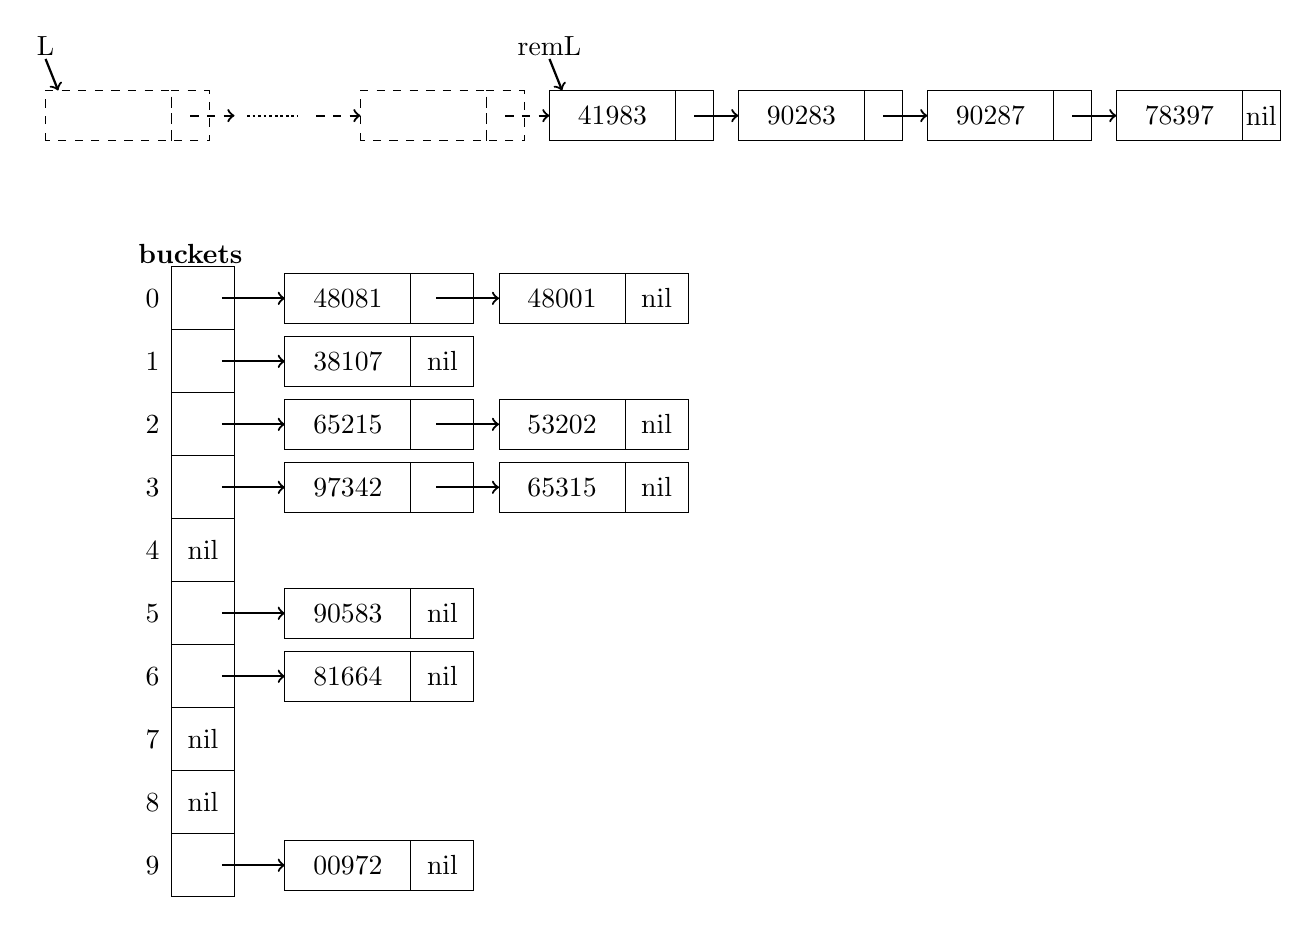
\begin{tikzpicture}[scale=0.8,place/.style={circle,draw, fill=white,inner sep=0pt,minimum size=5mm}]

        \foreach \x/\y in {-2/L, 6/remL}
            \draw (\x, 4.5) node {\y};
        \foreach \x in {-2, 6}
            \draw [thick, ->] (\x, 4.3) -- (\x+0.2, 3.8);

        \foreach \x in {-2, 3}
            \draw [dash pattern=on 3pt off 3pt] (\x, 3) rectangle (\x+2, 3.8) ;
        \foreach \x in {-2, 3}
            \draw [dash pattern=on 3pt off 3pt] (\x+2, 3) rectangle (\x+2.6, 3.8);
        \foreach \x in {-2, 0, 3}
            \draw [thick, ->, dash pattern=on 3pt off 3pt] (\x+2.3, 3.4) -- (\x+3, 3.4);
        \draw [thick, dash pattern=on 1pt off 1pt] (1.2, 3.4) -- (2, 3.4);

        \foreach \x in {6, 9, 12, 15}
            \draw (\x, 3) rectangle (\x+2, 3.8);
        \foreach \x/\y in {6/41983, 9/90283, 12/90287, 15/78397}
            \draw (\x+1, 3.4) node {\y};
        \foreach \x in {6, 9, 12, 15}
            \draw (\x+2, 3) rectangle (\x+2.6, 3.8);
        \foreach \x in {6, 9, 12}
            \draw [thick, ->] (\x+2.3, 3.4) -- (\x+3, 3.4);
        \draw (15+2.3, 3.4) node {nil};

        \draw (0.3, 1.2) node{{\textbf{buckets}}};
        \foreach \x in {0, ..., 9}
            \draw (-0.3, -\x*1+0.5) node{\x};
        \foreach \x in {0, ..., 9}
            \draw (0,-\x*1) rectangle (1,-\x*1+1);
        \foreach \x in {0, 1, 2, 3, 5, 6, 9}
            \draw [thick, ->] (0.8,-\x*1+0.5) -- (1.8,-\x*1+0.5);
        \foreach \x in {4, 7, 8}
            \draw (0.5,-\x*1+0.5) node {nil};

        \foreach \x in {0, 1, 2, 3, 5, 6, 9}
            \draw (1.8, -\x*1+0.5-0.4) rectangle (3.8,-\x*1+0.5+0.4);
        \foreach \x/\y in {0/48081, 1/38107, 2/65215, 3/97342, 5/90583, 6/81664, 9/00972}
            \draw (2.8, -\x*1+0.5) node {\y};
        \foreach \x in {0, 1, 2, 3, 5, 6, 9}
            \draw (3.8, -\x*1+0.5-0.4) rectangle (4.8,-\x*1+0.5+0.4);
        \foreach \x in {1, 5, 6, 9}
            \draw (4.3,-\x*1+0.5) node {nil};
        \foreach \x in {0, 2, 3}
            \draw [thick, ->] (4.2,-\x*1+0.5) -- (5.2,-\x*1+0.5);

        \foreach \x in {0, 2, 3}
            \draw (5.2, -\x*1+0.5-0.4) rectangle (7.2,-\x*1+0.5+0.4);
        \foreach \x/\y in {0/48001, 2/53202, 3/65315}
            \draw (6.2, -\x*1+0.5) node {\y};
        \foreach \x in {0, 2, 3}
            \draw (7.2, -\x*1+0.5-0.4) rectangle (8.2,-\x*1+0.5+0.4);
        \foreach \x in {0, 2, 3}
            \draw (7.7,-\x*1+0.5) node {nil};

        \end{tikzpicture}
    \caption{Radix Sort算法在分发第3个数字时的数据结构}
    \label{Fig:4_28DataStructOfRadix}
\end{figure*}

数据结构展示在图\ref{Fig:4_28DataStructOfRadix}中,图中显示的是
图\ref{Fig:RadixSort}例子中的第三步。注意每一个桶list都是逆序的,因为
新元素都是附加在list的前面。但是合并过程在合并的时候再次反转他们,所以
最后合并是正确的顺序。

\begin{algorithm}
基数排序

{\textbf{\emph{输入:}}}未排序list L,分发用的桶的数量radix,关键字分发
次数numFields。

{\textbf{\emph{输出:}}}排序的list, newL。

{\textbf{\emph{注意:}}}distribute过程反转桶中的lists,combine过程再次
反转它们(以逆序循环),所以合并完得到了想要的顺序。用List ADT的
操作来操作链表(参看图\ref{Fig:ListADTSpecification}).

\end{algorithm}

\begin{figure}
\begin{lstlisting}[language={Java},keywordstyle=\color{blue!70}, commentstyle=\color{red!50!green!50!blue!50}]
List radixSort(List L, int radix, int numFields){
    List[] buckets= newList[radix];
    int field;  // `关键字中域的数量`
    List newL;

    newL= L;
    for(field=0; field<numFields; field++){
        `将桶数组初始化为空;`
        distribute(newL, buckets, radix, field);
        newL=combine(buckets, radix);
    }
    return newL;
}
\end{lstlisting}
\end{figure}

\begin{figure}
\begin{lstlisting}[language={Java},keywordstyle=\color{blue!70}, commentstyle=\color{red!50!green!50!blue!50}]
void distribute(List L, list[] buckets, int radix, int field){
    List remL;
    remL=L;
    while(remL!=null){
        Element K=first(remL);
        int b=maskShift(field, radix, K.key);
        // `maskShift(f, r, key)选择key中第f个域(从右开始),`
        // `基于基数r。`
        // `结果b的范围是$0,\cdots, radix-1, b$是K所在的桶。`
        buckets[b]=cons(K, buckets[b]);
        remL= rest(remL):
    }
    return;
}
\end{lstlisting}
\end{figure}

\begin{figure}
\begin{lstlisting}[language={Java},keywordstyle=\color{blue!70}, commentstyle=\color{red!50!green!50!blue!50}]
List combine(List[] buckets, int radix){
    int b;  //`桶的数量`
    List L, remBucket;

    L= null;
    for(b= radix-1; b>=0; b--){
        remBucket=buckets[b];
        while(remBucket!=null){
            Key K= first(remBucket);
            L=cons(K, L);
            remBucket= rest(remBucket);
        }
    }
    return L;
}
\end{lstlisting}
\end{figure}

\subsubsection{分析与注意事项}
分发一个关键字需要解析出一个域,还有一个连接操作;步数是一个常数。所以对所有的
关键字,分发是$\Theta(n)$步。类似的,合并也是$\Theta(n)$步。分发和合并的趟数
是numFields,也是关键字分成多少个域。如果它可以控制在常数之内,基数排序总的
执行步数在n的线性时间之内。

我们的基数排序的实现使用了$\Theta(n)$的额外空间用于链域,提供的基数是以n相关的。
其它的不使用链的实现也将使用$\Theta(n)$的额外空间。
